\documentclass[a4paper,12pt]{report}
\usepackage{lgrind}
\pagestyle{plain}
\usepackage{amsmath,amsfonts,amssymb,amsthm}
\usepackage{listings}
\usepackage{cancel}
\usepackage{appendix}
\usepackage{fancyhdr}   
\usepackage{url}
\usepackage{path}
\usepackage[dvipdfm]{graphicx}
\usepackage{color}
\usepackage{array}
\usepackage{authblk}
\usepackage[margin=2cm, head=2cm, foot=1cm]{geometry}
\usepackage{verbatim}
\setlength{\topmargin}{-2.5cm}
\setlength{\textwidth}{17cm}
\setlength{\oddsidemargin}{-0.5cm}
\setlength{\evensidemargin}{-0.5cm}
\setlength{\textheight}{22.5cm}
\setlength{\footskip}{1cm}
\renewcommand{\topfraction}{0.9}
\renewcommand{\bottomfraction}{0.8}
\setcounter{topnumber}{2}
\setcounter{bottomnumber}{2}
\setcounter{totalnumber}{4}
\usepackage{hyperref}
\usepackage{pdfpages}
\lstset{columns=fullflexible,basicstyle=\ttfamily}


\renewcommand{\floatpagefraction}{0.9}%

\newcommand{\ROOT}{{\ttfamily ROOT}}
\newcommand{\CINT}{{\ttfamily CINT}}
\newcommand{\CPP}{{\ttfamily C++}}
\newcommand{\gpp}{{\ttfamily g++}}
\newcommand{\clang}{{\ttfamily clang}}
\newcommand{\php}{{\ttfamily php}}
\newcommand{\psql}{{\ttfamily PostgreSQL}}
\newcommand{\python}{{\ttfamily python}}
\newcommand{\PyROOT}{{\ttfamily PyROOT}}
\newcommand{\larlight}{{\ttfamily LArLight}}
\newcommand{\larsoft}{{\ttfamily LArSoft}}
\newcommand{\git}{{\ttfamily git}}
\newcommand{\doxygen}{{\ttfamily doxygen}}
\newcommand{\HTML}{{\ttfamily HTML}}
\newcommand{\ART}{{\ttfamily ART}}
\newcommand{\enum}{{\ttfamily enum}}
\newcommand{\psycopg}{{\ttfamily psycopg2}}
\newcommand{\aptget}{{\ttfamily apt-get}}
\newcommand{\yum}{{\ttfamily yum}}
\newcommand{\fink}{{\ttfamily fink}}
\newcommand{\brew}{{\ttfamily home brew}}
\newcommand{\macport}{{\ttfamily macport}}
\newcommand{\xcode}{{\ttfamily Xcode}}
\newcommand{\hstore}{{\ttfamily HSTORE}}
\newcommand{\procdb}{{\ttfamily procdb}}
\newcommand{\dstream}{{\ttfamily dstream}}
\newcommand{\pubdbi}{{\ttfamily pub\_dbi}}
\newcommand{\pubutil}{{\ttfamily pub\_util}}
\newcommand{\pubsmtp}{{\ttfamily pub\_smtp}}
\newcommand{\publogger}{{\ttfamily pub\_logger}}
\newcommand{\pubexception}{{\ttfamily pub\_exception}}
\newcommand{\stdout}{{\ttfamily stdout}}
\newcommand{\stderr}{{\ttfamily stderr}}
\newcommand{\pubs}{{\ttfamily pubs}}
\newcommand{\sql}{{\ttfamily SQL}}



\begin{document}

\title{PUBS: Data Processing Software Framework}
%\date{March 12th, 2014}
\author{
  Kazuhiro Terao, kazuhiro@nevis.columbia.edu
}
\maketitle

\begin{abstract}
This document describes about {\python/\php/\psql} UBooNE Software (a.k.a. \pubs) framework
written for online data processing of the experiment. Each step of data processing, defined
as a ``project'', carries a project-specific category of {\it state} and corresponding 
actions to deliver data to a next step. Projects' state are stored in {\psql} database server
with a dedicated procedures for data queries. {\pubs} provides a generic, {\python} based software 
framework for development of ``project'' code. In addition, it provides necessary tools for
project execution including a daemon program for parallel project execution and framework logger
system. Monitoring of project execution is realized through a web-browser using a {\php} based 
toolkit, which can be also used for experts to actively interface with currently running projects.
Finally this document assumes you have a modest knowledge about {\python} and common programming 
terminologies. 
\end{abstract}

% Table of Contents
\tableofcontents

\newpage

% Prep
\chapter{Preparation}
\label{prep}

This chapter describes about building blocks of {\pubs} framework. Sec.\ref{pubs:model} covers the data process management model and the framework design.
Three following sections \ref{pubs:psql}, \ref{pubs:python}, \ref{pubs:php}
 cover {\psql}, {\python}, and {\php} components as building blocks of the 
framework respectively. More practical development how-to's are discussed 
in the next chapter.

\section{Data Processing Model}
\label{pubs:model}

{\pubs} is a data processing software framework that supports a specific
data process model implementation by application developers. In particular,
it has following features:
\begin{itemize}
  \item Use {\psql} for process management
  \item Supports {\python} code development for implementation
  \item Provides {\php} toolkit for application management and monitoring
\end{itemize}
This section describes a generic idea of {\pubs} data processing model.

\subsection{Project: A Unit Task of Data Processing}
\label{pubs:model:project}
A typical model of data processing is a well defined chain of processes
in which a particular process is triggered by a completion or an initiation
of another process. For instance, the end of running DAQ may trigger a file
transfer protocole to move a raw data file to a storage server. In {\pubs},
each of such processes is called a {\it project}. 

\subsubsection{Project Status}
Each {\pubs} project carries a specific {\it status} code represented
by an integer. A unit of status is defined by, in case of MicroBooNE, a
unique combination of four integeres: run, sub-run, {\it sequence} 
(or simply {\it seq}), and the project version number. This combination is
referred to as {\it TaskID} in this document. A run and sub-run numbers 
defines a boundary of data taking  defined by a DAQ as you might guess. 
A sequence number, on the other hand, is a possible sub-set of run and 
sub-run number combination, and is defined by a project. It is there to 
support some projects that may need to sub-divide a process to deal with 
a particular DAQ run. As its name says, the project version is an integer
representing different version of the same project. 

Each {\pubs} project carries a status for each TaskID. Special status code 
1 is reserved to represent the initial status for any project. Similarly, 
code 0 is reserved to represent the completion status for any 
project. Any other integer values may be used to represent various status 
which meaning may be defined by a project.

\subsubsection{Project Version}
One important feature of data processing framework is an ability to roll-back
and re-process some older data files. Reprocessing of data is supported in
{\pubs}, but it requires to change a project version number. The basic 
assumption for forcing the version update for re-processing is that something
must have changed to roll back and re-process data. 
\begin{figure}[ht]\begin{center}
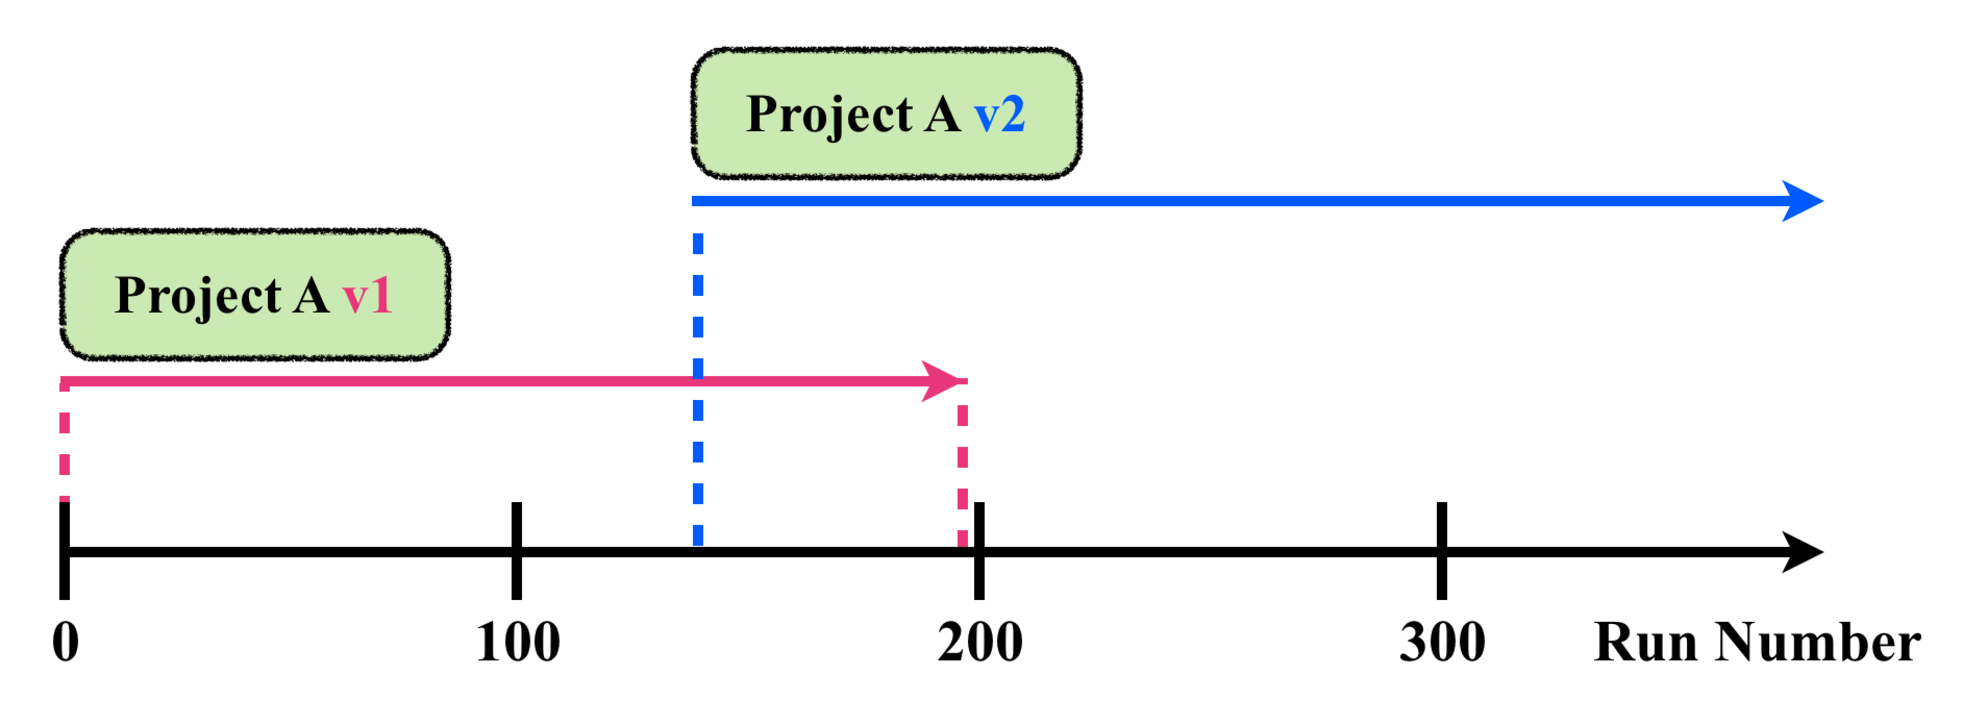
\includegraphics[width=14cm]{./img/PUB_ProjectVersion.pdf}
\caption{ Example diagram showing how project version may be used. 
The horizontal axis shows the time in the unit of a run number 
(sub-run number ignored for simplicity). The diagram shows that the 1st 
version of project A processing data up to around run 200. Then the updated 
2nd version starts re-processing runs just before around run 150 and takes 
over to process all future runs.}
\label{pubs:model:version}
\end{center}\end{figure}
Figure\ref{pubs:model:version} shows an example of reprocessing associated
with a specific project's version update.


\subsubsection{Project Table}
Each project status is stored in {\psql} database table with a name same
as the project's name, called a project table. For this reason, {\bf a 
project name must be unique}. A project table contains several information 
per unique combination of run, sub-run, seq numbers, and they are shown below 
with corresponding {\psql} data type.
\begin{itemize}
\item Run $\ldots$ INT $\ldots$ DAQ run number
\item SubRun $\ldots$ INT $\ldots$ DAQ sub-run number
\item Seq $\ldots$ SMALLINT $\ldots$ project sequence number
\item Status $\ldots$ SMALLINT $\ldots$ project status code
\item Data $\ldots$ TEXT $\ldots$ Generic ``data'' associated with a particular run, sub-run combination
\item ProjectVer $\ldots$ SMALLINT $\ldots$ a version number for a project
\end{itemize}
A project may record some ``data'' in string representation for each TaskID.
However, it is recommended to avoid to store such information when possible 
as this makes the table size to become larger. Finally, as mentioned before,
a project is allowed to have a different version number. 

\subsubsection{Project Execution Model}
Each project is expected to have a single {\python} script to be executed.
This {\python} script should fetch an array of target TaskID from the 
database based on a status code. Depending on the status code, then, the
script may take a certain action, and possibly update the status code in the
database upon success. In short, the status code is used as a trigger for
a specific action by projects. 

Now, information needed to execute each such script is called {\it project
information}, and is stored in a separate database table called the 
{\it ProcessTable}. In the next section, we discuss about this table and
also a machinary to automatically execute a project's {\python} script
using a daemon tool.

\subsection{ProcessTable And Daemon Execution}
\label{pubs:model:daemon}
Information about individual project is stored in a dedicated database
table called ``ProcessTable''. Unlike project tables that exist one per
project, this is a unique table in the database that holds all projects'
information. The table schema is shown below:
\begin{itemize}
  \item ID $\ldots$ SERIAL $\ldots$ a unique integer key for each project
  \item Project $\ldots$ TEXT $\ldots$ the name of a project
  \item ProjectVer $\ldots$ SMALLINT $\dots$ the version number of a project
  \item Command $\ldots$ TEXT $\ldots$ a project execution command to be run
  \item Frequency $\ldots$ INT $\ldots$ latency in seconds between each execution of a project
  \item EMail $\ldots$ TEXT $\ldots$ email contact(s) in case of a trouble
  \item StartRun $\ldots$ INT $\ldots$ the first run-number to be processed
  \item StartSubRun $\ldots$ INT $\ldots$ the first sub-run number to be processed
  \item Resource $\ldots$ HSTORE $\ldots$ a dynamic string-to-string map data container
  \item Enabled $\ldots$ BOOLEAN $\ldots$ a boolean flag for project execution (only if it is true)
  \item Running $\ldots$ BOOLEAN $\ldots$ a boolean flag enabled during project execution
  \item LogTime $\ldots$ TIMESTAMP $\ldots$ a time-stamp logged per entry update
\end{itemize}
where, among many self-descriptive columns, ``Resource'' column holds HSTORE
type variable that can be used to store any project-specific information.
Such information includes, for example, the path to a specific data directory
and expected file name format that requires run and sub-run numbers such as
\begin{center}
 {\ttfamily Run\%05d\_SubRun\%03d.bin}.
\end{center}
with which your project can figure out the expected file name for a given
TaskID (i.e. run and sub-run numbers). 

Note that storing such information in ProcessTable is much lighter than 
storing the actual filename in a project table's ``Data'' column because 
the ``Data'' column stores information for every single TaskID while 
ProcessTable entry is made only one per project. Again, store as much
information as possible in ProcessTable and avoid using ``Data'' column
of a project table when possible.

\subsubsection{Daemon: Master Scheduler}
An execution of a project should be as simple as:
\begin{lstlisting}
  > python my_project.py
\end{lstlisting}
where my\_project.py is the executor of a project. In {\pubs}, however,
there is a simple daemon project management tool that periodically 
looks up the ProcessTable and executes the enabled projects in parallel. 
So it is a lot like {\ttfamily cron} in Unix/Linux but with a process
manager aspect.  

The daemon process is responsible for project management: it keeps track
of history of running each project, and it ensures its resoure usage. 
The project information is updated every 120 seconds (configurable) and 
synchronized with the ProcessTable contents in the database. An expert
can impose a change in project information without interrupting the daemon
process. Another important role of the daemon is to keep the integrity of
the DAQ's run table with all enabled projects' table. Once in every 300
seconds (configurable), the daemon process synchronizes run and sub-run
number entries in each project table and match with the DAQ run table.

That being said, it is extremely important that each project is a truly
modulated action, and does not depend on an execution by the daemon. In
other words, one should be able to always run a project by simply invoking
from a command line. This allows us to take any emergency treatment when,
somehow, the daemon procedure cannot be used.

\begin{figure}\begin{center}
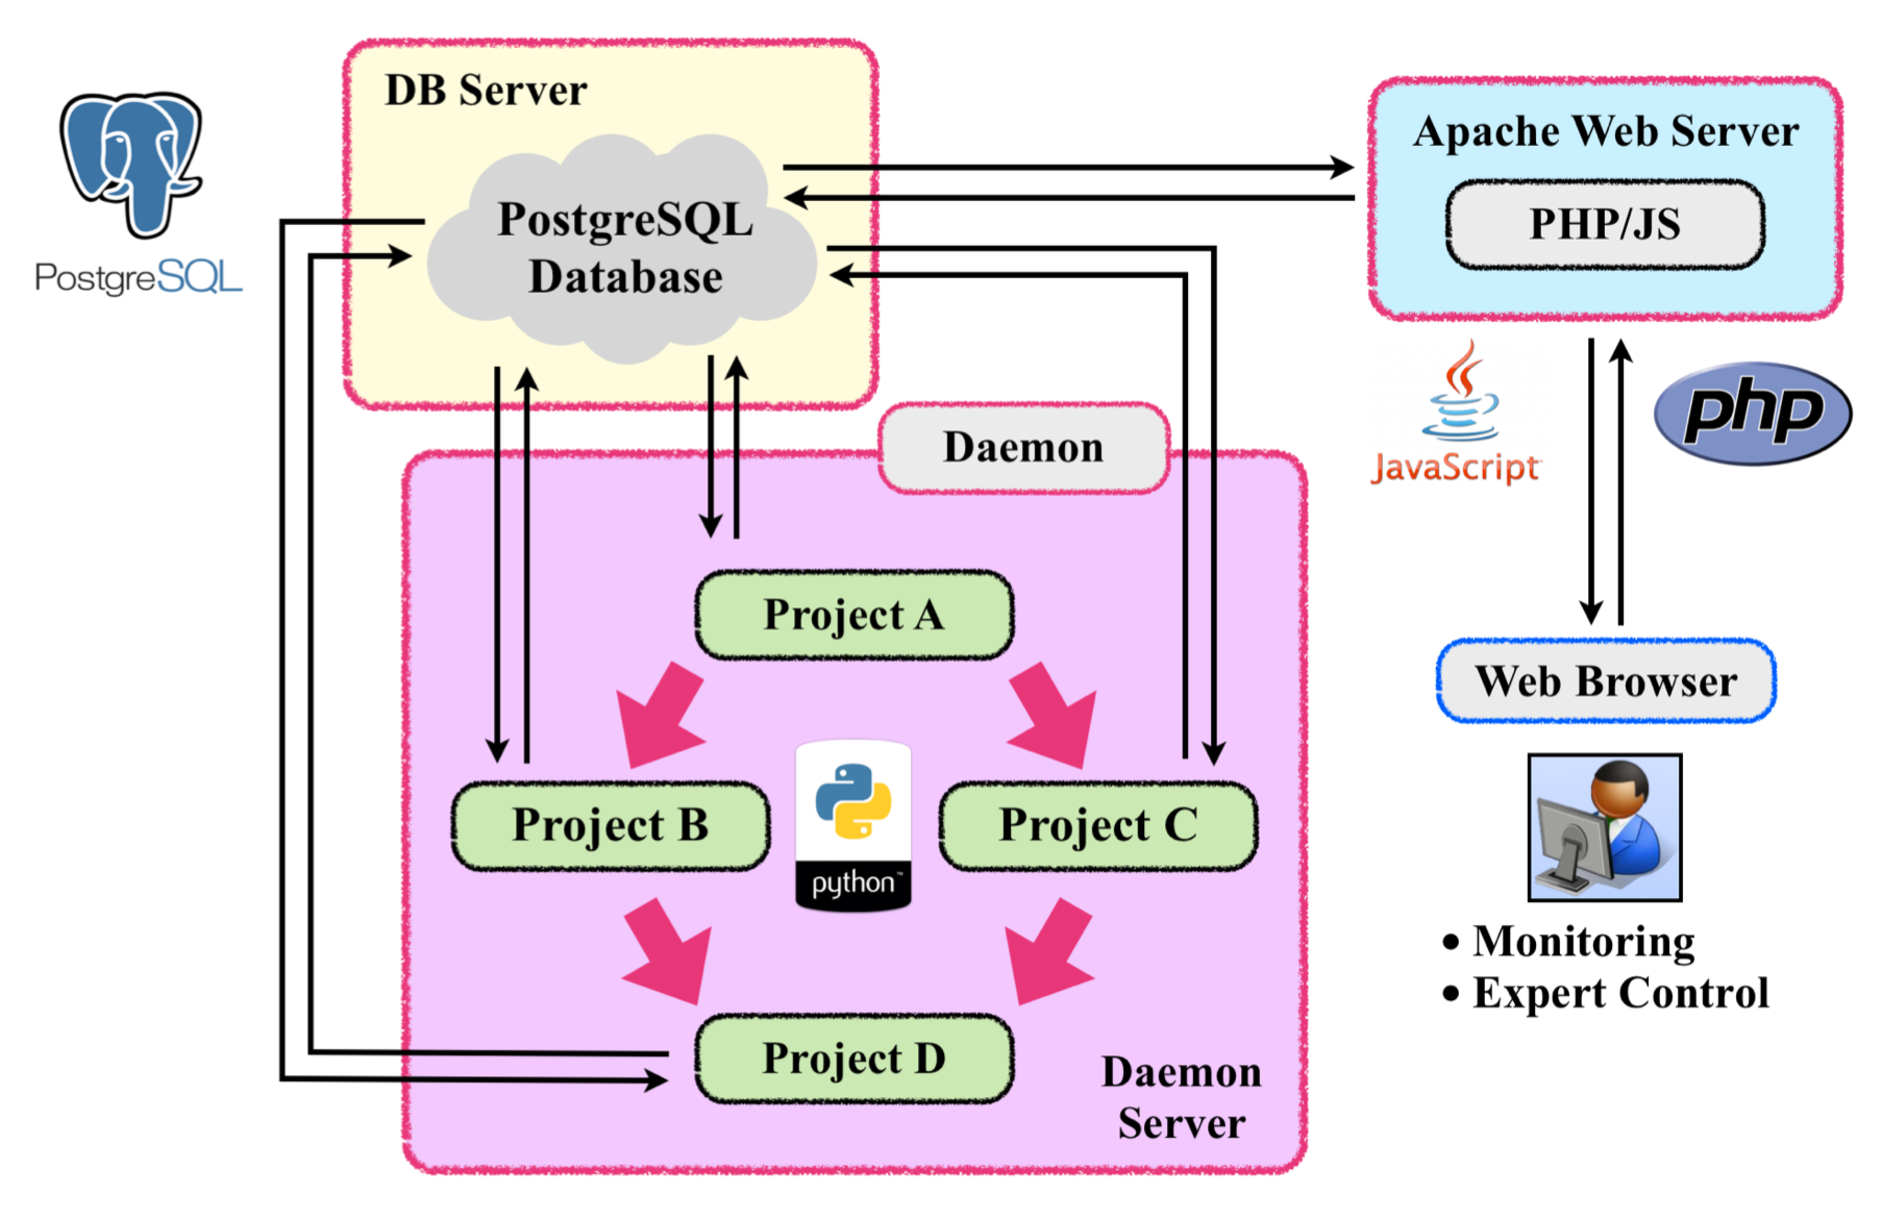
\includegraphics[width=14.5cm]{./img/PUB_Model.pdf}
\caption{ An abstract drawing that shows how data flows into and from the
{\psql} database within {\pubs} framework. Each project and daemon process
all talk to the database server. The {\php} web-interface provides monitoring
and project management tools.}
\label{pubs:model:model}
\end{center}\end{figure}


\subsection{Web Monitoring And Process Management}
\label{pubs:model:monitor}

Figure\ref{pubs:model:model} shows a brief data flow from and into the 
{\psql} database. As described in Sec.\ref{pubs:model:project} and
\ref{pubs:model:daemon}, each project and daemon accesses the database
server individually. In addition to the project execution framework, 
{\pubs} provides {\php} based monitoring and management interface through 
a web server machine and end-user's web browser application. Accordingly
there is a database connection between the web server and {\psql} server
machines.

The capability to monitor each projects' status through a web browser is
quite useful for a routine inspection, such as shifters' check list.
Similarly a formatted control pannel for managing project
execution is useful for experts to take action without logging into the
machine. The details of {\php} implementation is quite experiment specific, 
and the MicroBooNE usage will be discussed in Ch.\ref{dstream}. 


\section{{\psql} Functions}
\label{pubs:psql}

Now that we spent many pages to discuss about the {\pubs} model, let's talk
about something real and practical. This section presents a list of {\pubs} 
functions implemented on the {\psql} server. About a half of them are for
experts' use (in fact mostly for daemon and automated scripts since human
hands are one of last things to be trusted), and the other half is for
project scripts to use. 

If you are a project code developper and do not find a function of your
need, please contact the author and he will be more than happy to assist
how the existing function may solve the problem or implement a brand
new function to make your life easier.

\subsection{Project Information/Status Query}
These are functions that can be used by projects upon execution. That being
said, however, it is {\bf \color{blue} strongly recommended to use {\python} 
API within {\pubs} to execute these functions}. They should not be executed
from {\psql} interpreter or directly executing from an SQL script. If the 
list lacks any function needed for a project execution, please contact the 
author with a request. Functions and corresponding {\python} API will be 
provided.
\begin{itemize}
  \item {\bf DoesTableExist( name TEXT )}
    \begin{itemize}
      \item Checks if a table of the {\it name} exists or not in the database
        by checking the administrative master table. The table name is required
        to be in lowercase (there is no uppercase vs. lowercase in distinction
        among {\psql} server objects).
    \end{itemize}
  \item {\bf DoesProjectExist( name TEXT )}
    \begin{itemize}
      \item Checks if a project with the {\it name} exists or not in the 
        database. In addition to DoesTableExist(), this function checks
        if a specified project exists or not.
    \end{itemize}
  \item {\bf GetRunTimeStamp( Run INT, SubRun INT )}
    \begin{itemize}
      \item A function to retrieve the run start and end time stamp.
    \end{itemize}
  \item {\bf ProjectResource( name TEXT )}
    \begin{itemize}
      \item Returns a project resource (information needed for an execution)
        for a specified project name.
    \end{itemize}
  \item {\bf IncreaseProjSequence( name TEXT, run INT, subrun INT, nseq
    SMALLINT, status SMALLINT) }
    \begin{itemize}
      \item Increase number of sequence count in the specified project table
        for the specified run/sub-run number combination. Input status code 
        is used for all newly created TaskIDs.
    \end{itemize}
  \item {\bf UpdateProjStatus( name TEXT, run INT, subrun INT, seq SMALLINT,
    status SMALLINT, data TEXT)}
    \begin{itemize}
      \item Update the specified project's status for the specified TaskID. 
        At the same time, a TaskID specific data can be also stored although
        that is not necessary (by default the last argument is set to NULL).
    \end{itemize}
  \item {\bf GetProjectData( name TEXT, run INT, subrun INT, seq SMALLINT )}
    \begin{itemize}
      \item Retrieve project data for a specified TaskID. Only accessible to
        The data from the latest version number to avoid a confusion (and
        hence version number cannot be specified).
    \end{itemize}
  \item {\bf GetRuns( name TEXT, status SMALLINT) }
    \begin{itemize}
      \item Returns a table of TaskID (run, sub-run, seq., project-version) 
        for which the specified project carries the specified status code.
    \end{itemize}
  \item {\bf GetRuns( TEXT[]::ARRAY, SMALLINT[]::ARRAY )}
    \begin{itemize}
      \item Similar to GetRuns and it returns a table of run/sub-run number 
      combinations for which all specified projects in the first argument
      carry specified status code in the second argument. This function
      is useful to obtain a list of run/sub-run numbers across multiple
      project tables for specific combination of status code. Because 
      a sequence number is project dependent, it returns run/sub-run for
      which all belonging sequence status uniquely matches with the specified
      status code.
    \end{itemize}

\end{itemize}


\subsection{Functions For Project Management}
These are functions to be used by daemon process to maintaine/running the
projects. In principle these should not be used by a project execution. 
\begin{itemize}
  \item {\bf RemoveProject( name TEXT )} 
    \begin{itemize}
      \item Properly remove a project: drop a project table and remove the
        project information entry from the ProcessTable.
    \end{itemize}
  \item {\bf ListProject()}
    \begin{itemize}
      \item List all projects with the latest version number from ProcessTable.
    \end{itemize}
  \item {\bf ListEnabledProject()}
    \begin{itemize}
      \item List currently enabled project information with the latest version
        number from the ProcessTable.
    \end{itemize}
  \item {\bf DefineProject( name TEXT, command TEXT, frequency INT, email TEXT,
    start\_run INT, start\_subrun INT, resource HSTORE, enabled BOOLEAN )}
    \begin{itemize}
      \item A function to define a new project. It takes in project information
        and registers into the ProcessTable. It also calls {\bf MakeProjTable}
        function to create a project table.
    \end{itemize}
  \item {\bf MakeProjTable( name TEXT )}
    \begin{itemize}
      \item Function dedicated to create a project table. This function is
        to be called by {\bf DefineProject} and not to be called by hand!
    \end{itemize}
  \item {\bf UpdateProjectConfig( name TEXT, command TEXT, frequency INT, email
    TEXT, resource HSTORE, enabled BOOLEAN, version INT)}
    \begin{itemize}
      \item A function to alter and update project configuration. As seen in
        the function arguments, start run/sub-run number cannot be altered by
        design.
    \end{itemize}
  \item {\bf ProjectVersionUpdate( name TEXT, command TEXT, frequency INT,
    email TEXT, run INT, subrun INT, resource HSTORE, enable BOOLEAN)}
    \begin{itemize}
      \item Increment the project version number and store new project
        information. Unlike {\bf UpdateProjectConfig}, this function can
        register any project information as there will be a distinct row
        to be inserted in the ProcessTable.
    \end{itemize}
  \item {\bf GetVersionRunRange( name TEXT )}
    \begin{itemize}
      \item For a specified project name, returns multiple result sets each
        representing a specific run number range with the corresponding
        project version number.
    \end{itemize}
  \item {\bf InsertIntoProjTable( name TEXT, run INT, subrun INT )}
    \begin{itemize}
      \item Insert a new run/sub-run number entry into a project table with
        the default status code of 1. The latest version number for the
        subject run/sub-run is also taken from the ProcessTable.
    \end{itemize}
  \item {\bf OneProjectRunSynch()}
    \begin{itemize}
      \item Make sure one particular project table has run/sub-run 
        numbers that currently appears in the MainRun table and above
        the specified run/subrun numbers in the argument.
    \end{itemize}
  \item {\bf AllProjectRunSynch()}
    \begin{itemize}
      \item Make sure all project table has run/sub-run numbers that 
        currently appears in the MainRun and above the specified start
        run/sub-run numbers in the project information.
    \end{itemize}
  \item {\bf ProjectInfo(name TEXT, ver INT)}
    \begin{itemize}
      \item Returns project information for a specified version number.
        By default the version number does not need to be specified.
        If not given, it is set to the latest version number. This function
        is used to run a project via daemon.
    \end{itemize}
\end{itemize}

\subsection{Admin Functions}
Functions prepared for the top-level administrative purposes. These functions
should be executed by database admins only.
\begin{itemize}
  \item {\bf RemoveProcessDB()}
    \begin{itemize}
      \item ``Properly'' remove {\it everything}. This function drops all
        projects registered in ProcessTable using {\bf RemoveProject} 
        function. Then it drops an empty ProcessTable.
    \end{itemize}
  \item {\bf CreateProcessTable()}
    \begin{itemize}
      \item A simple function to create the ProcessTable.
    \end{itemize}
  \item {\bf CreateTestRunTable()}
    \begin{itemize}
      \item A function to create ``fake'' MainRun table. This is for 
        development work, and not for an official operation. In the official
        production, MainRun table is slave-copied from the configuration
        database automatically.
    \end{itemize}
  \item {\bf InsertIntoTestRunTable( Run INT, SubRun INT, TimeStart TIMESTAMP, TimeEnd TIMESTAMP )}
    \begin{itemize}
      \item A function to insert a new entry into the ``fake'' MainRun table.
        This is not meant to be used for the offial production.
    \end{itemize}
  \item {\bf FillTestRunTable( NRuns INT, NSubRuns INT)}
    \begin{itemize}
      \item A function to fill the ``fake'' MainRun table with multiple entries
        at once. It fills the table with NRuns, each with NSubRuns.
    \end{itemize}
  \item {\bf CheckDBIntegrity()}
    \begin{itemize}
      \item Returns a boolean after checking the process DB integrity. 
        In particular it checks if ProcessTable exists or not, and then
        checks if all projects registered in ProcessTable have own project
        tables.
    \end{itemize}
\end{itemize}





\section{{\python} Software Framework}
\label{pubs:python}
The ``software framework'' part of {\pubs}, which provides the code base 
for application development, is really in {\python}. This section describes
 {\python} tools in {\pubs} that can be used to develop a project execution 
code and set up the data processing chain of multiple projects.

There are three (somewhat) big {\python} modules in {\pubs}:
\begin{itemize}
  \item {\pubutil} $\ldots$ basic framework tools
  \item {\pubdbi} $\ldots$ generic database interface based using {\psycopg}
  \item {\dstream} $\ldots$ data processing framework toolkit
\end{itemize}
A project code developer interfaces with {\dstream} directly while that itself 
depends on basic tools defined in {\pubutil} and {\pubdbi}. We go over each 
of these in the following sections. 

\subsection{{\pubutil}: Basic Toolkit}
This module introduce 3 objects: {\publogger}, {\pubsmtp}, and {\pubexception}.
They are framework logging tool, email sender function via SMTP, and a base exception
class definition. 

\subsubsection{{\publogger} $\ldots$ Logging Module}
This is the framework logger tool, and uses a popular {\python}'s logging module.
{\publogger} is a factory class that can instansiate an individual logger instance
with a specific message format and a choice of stream: either {\stdout}/{\stderr} or
output file stream. 

Each logger instance created by {\publogger} factory has a unique name, and 
can be instantiated by a factory function call:
\begin{lstlisting}
  >>> pubs_logger.get_logger('my_logger')
\end{lstlisting}
for a logger named ``my\_logger''. {\publogger} keeps track of all created loggers 
in its class variable {\ttfamily \_loggers}. When there is a request for a logger
with the same name created in the past, it returns the same instance.
\begin{lstlisting}
  >>> from pub_util import pub_logger
  >>> pub_logger.get_logger('a')
  [ INFO    ] pub_logger (L: 81 ) >> {_add_logger} OPENED LOGGER a
  <logging.Logger object at 0x10b903f90>
  >>> pub_logger.get_logger('a')
  <logging.Logger object at 0x10b903f90>
  >>>
\end{lstlisting}

As you might expect in any similar tool, {\publogger} has several message levels:
debug, info, warning, error, and critical. The default message level is set via
shell environment variable {\ttfamily \$PUB\_LOGGER\_LEVEL}, which is automatically
set in {\ttfamily setup.sh} configuration script. You may change the level if you
wish. You do not have to change the configuration script, but instead just change
the shell environment variable in any way you want (for instance by hand on your
terminal instead of sourcing a script). The set shell environment value is parsed 
in {\ttfamily pub\_util/pub\_env.py} script to an appropriate value. 
Similarly, the stream destination (either {\stdout} or file stream) is
set via shell environment variable {\ttfamily \$PUB\_LOGGER\_DRAIN}, again set
automatically in {\ttfamily setup.sh}. In case the drain is chosen to be a text
file stream, {\ttfamily \$PUB\_LOGGER\_FILE\_LOCATION} environment variable's value
is used as the log file location.

Each message level has a dedicated logger function call to parse an output message
through your logger. Here is an example of formatted output :
\begin{lstlisting}
  >>> a.debug('This is debug')
  [ DEBUG   ] <stdin> (L: 1  ) >> {<module>} This is debug
  >>> a.info('This is info')
  [ INFO    ] <stdin> (L: 1  ) >> {<module>} This is info
  >>> a.warning('This is warning')
  [ WARNING ] <stdin> (L: 1  ) >> {<module>} This is warning
  >>> a.error('This is error')
  [ ERROR   ] <stdin> (L: 1  ) >> {<module>} This is error
  >>> a.critical('This is critical')
  [ CRITICAL] <stdin> (L: 1  ) >> {<module>} This is critical
\end{lstlisting}
The logger specifies the message level, and prints out three more information in
addition to the sent message by the caller. The first `$<$stdin$>$' tells where the
message is sent from. `(L: 1  )' tells us which line in the caller's module code
this function is called from. Then `\{$<$module$>$\}' tells us the name of the
caller's module. In the above example, this is called from the main, and hence
it is not really useful. However, these information help us to track down problems
easily as you can identify where each function call is made. For instance, running
{\ttfamily ds\_daemon.py} to test the installation (see Sec.\ref{prep:pubs:daemon}),
you have probably seen this message:
\begin{lstlisting}
  [ DEBUG   ] ds_daemon (L: 128) >> {load_projects} Updating project dummy_daq ...
\end{lstlisting}
 This menas that a logger function ``debug'' was called by a function 
{\ttfamily load\_projects} and the exact location is in line number 128 of the 
module code {\ttfamily ds\_daemon.py}. 

\subsubsection{{\pubsmtp} $\ldots$ Simple SMTP Protocole}
{\pubsmtp} is a simple function that uses the Simple Mail Transfer Protocole to
send an email message. One can specify the recipients, subject and text message
to be sent. By default, the SMTP account, server address (and port), and password
 are taken from, again, shell environment variables: {\ttfamily \$PUB\_SMTP\_ACCT}, 
{\ttfamily \$PUB\_SMTP\_SRVR}, and {\ttfamily \$PUB\_SMTP\_PASS} respectively.
These are currently set to an email account created for a common use. You may change
this to your account if you wish, or we use an official account when in production.

\subsubsection{{\pubexception} $\ldots$ Simple Exception}
This is an exception class that inherits from the base {\python} {\ttfamily Exception}.
It is nothing special but takes an error message in the constructor argument.
Only purpose is to have a common exception within {\pubs} so that we can catch {\pubs}
specific exception.

\subsection{{\pubdbi}: Generic DB Interface}
{\pubdbi} module defines client tools used to interface with {\psql} database server.
In particular it contains following classes
\begin{itemize}
  \item {\pubdbconn} $\ldots$ for connecting database server
  \item {\pubdbdata} $\ldots$ class that encapsulates connection information 
  \item {\pubdbexception} $\ldots$ exception dedicated for {\pubdbi} module
  \item {\pubdbreader} $\dots$ ``read-only'' database query API instantiated by {\pubdbconn}
  \item {\pubdbwriter} $\dots$ ``read/write'' database query API instantiated by {\pubdbconn}
\end{itemize}
Note that a project code developer should use a wrapper API that is under {\dstream}.
This section covers base components that are usually hidden in behind.
OK let's go through them. Hope I can contribute to your good sleep.

\subsubsection{{\pubdbconn} database connection factory}
This is a factory class that connects to the database using {\psycopg} and generate
a connection cursor ({\ttfamily psycopg2.cursor}) for {\pubdbreader} and {\pubdbwriter}
APIs.

\subsection{{\dstream}: Data Processing Framework}


\section{{\php}-based Web Interface}
\label{pubs:php}
\input{./src/PUBS/php}




% Introduction
\chapter{Basic of {\pubs}}
\label{pubs}

This chapter describes about building blocks of {\pubs} framework. Sec.\ref{pubs:model} covers the data process management model and the framework design.
Three following sections \ref{pubs:psql}, \ref{pubs:python}, \ref{pubs:php}
 cover {\psql}, {\python}, and {\php} components as building blocks of the 
framework respectively. More practical development how-to's are discussed 
in the next chapter.

\section{Data Processing Model}
\label{pubs:model}

{\pubs} is a data processing software framework that supports a specific
data process model implementation by application developers. In particular,
it has following features:
\begin{itemize}
  \item Use {\psql} for process management
  \item Supports {\python} code development for implementation
  \item Provides {\php} toolkit for application management and monitoring
\end{itemize}
This section describes a generic idea of {\pubs} data processing model.

\subsection{Project: A Unit Task of Data Processing}
\label{pubs:model:project}
A typical model of data processing is a well defined chain of processes
in which a particular process is triggered by a completion or an initiation
of another process. For instance, the end of running DAQ may trigger a file
transfer protocole to move a raw data file to a storage server. In {\pubs},
each of such processes is called a {\it project}. 

\subsubsection{Project Status}
Each {\pubs} project carries a specific {\it status} code represented
by an integer. A unit of status is defined by, in case of MicroBooNE, a
unique combination of four integeres: run, sub-run, {\it sequence} 
(or simply {\it seq}), and the project version number. This combination is
referred to as {\it TaskID} in this document. A run and sub-run numbers 
defines a boundary of data taking  defined by a DAQ as you might guess. 
A sequence number, on the other hand, is a possible sub-set of run and 
sub-run number combination, and is defined by a project. It is there to 
support some projects that may need to sub-divide a process to deal with 
a particular DAQ run. As its name says, the project version is an integer
representing different version of the same project. 

Each {\pubs} project carries a status for each TaskID. Special status code 
1 is reserved to represent the initial status for any project. Similarly, 
code 0 is reserved to represent the completion status for any 
project. Any other integer values may be used to represent various status 
which meaning may be defined by a project.

\subsubsection{Project Version}
One important feature of data processing framework is an ability to roll-back
and re-process some older data files. Reprocessing of data is supported in
{\pubs}, but it requires to change a project version number. The basic 
assumption for forcing the version update for re-processing is that something
must have changed to roll back and re-process data. 
\begin{figure}[ht]\begin{center}
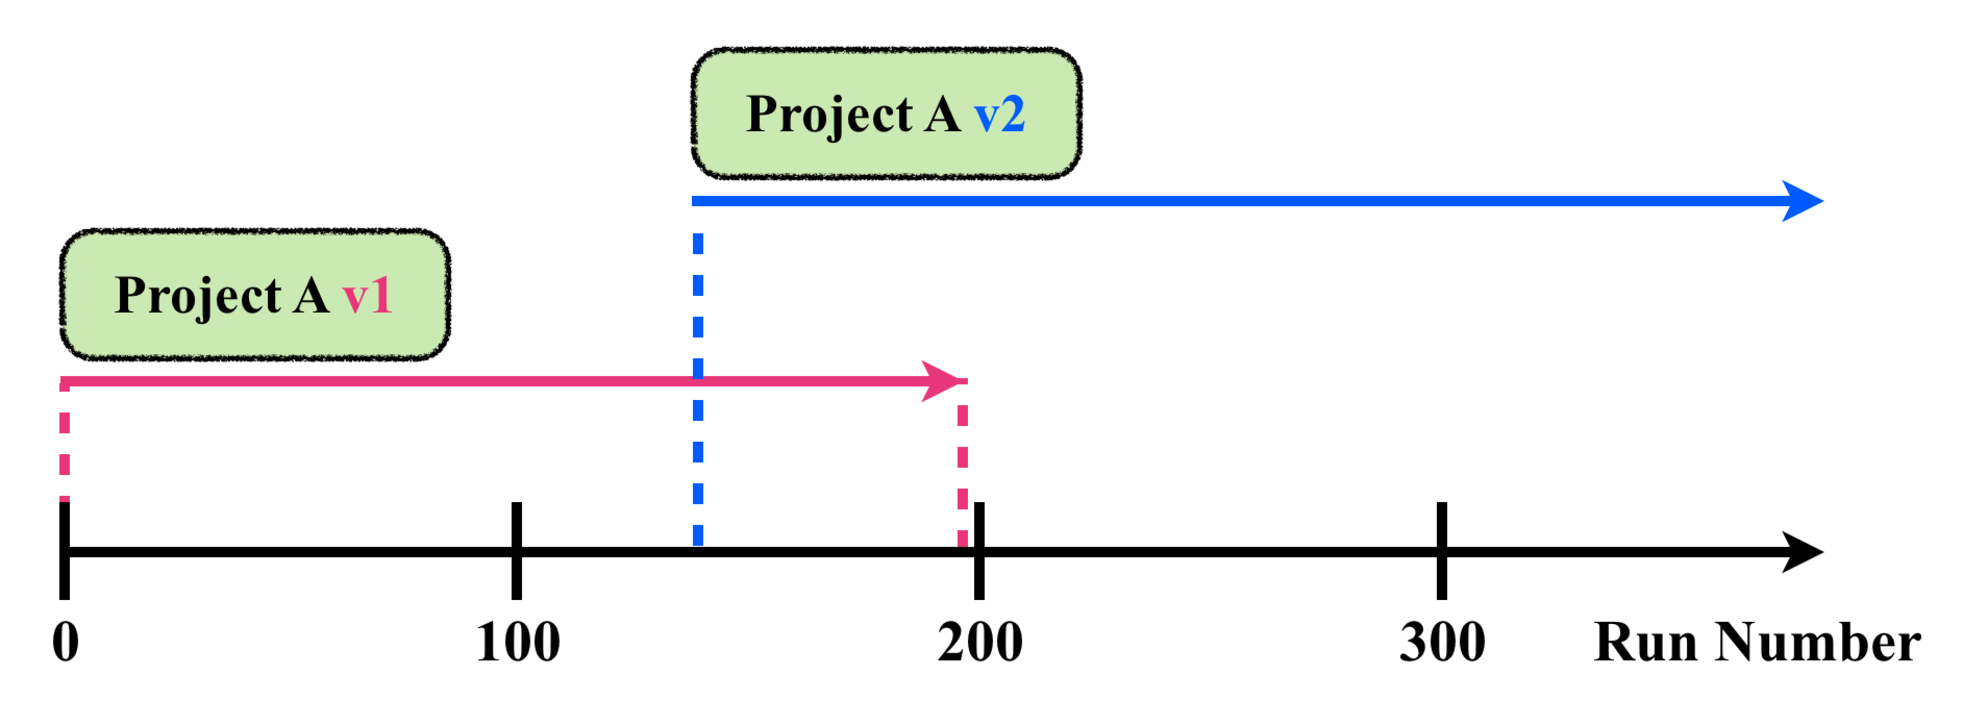
\includegraphics[width=14cm]{./img/PUB_ProjectVersion.pdf}
\caption{ Example diagram showing how project version may be used. 
The horizontal axis shows the time in the unit of a run number 
(sub-run number ignored for simplicity). The diagram shows that the 1st 
version of project A processing data up to around run 200. Then the updated 
2nd version starts re-processing runs just before around run 150 and takes 
over to process all future runs.}
\label{pubs:model:version}
\end{center}\end{figure}
Figure\ref{pubs:model:version} shows an example of reprocessing associated
with a specific project's version update.


\subsubsection{Project Table}
Each project status is stored in {\psql} database table with a name same
as the project's name, called a project table. For this reason, {\bf a 
project name must be unique}. A project table contains several information 
per unique combination of run, sub-run, seq numbers, and they are shown below 
with corresponding {\psql} data type.
\begin{itemize}
\item Run $\ldots$ INT $\ldots$ DAQ run number
\item SubRun $\ldots$ INT $\ldots$ DAQ sub-run number
\item Seq $\ldots$ SMALLINT $\ldots$ project sequence number
\item Status $\ldots$ SMALLINT $\ldots$ project status code
\item Data $\ldots$ TEXT $\ldots$ Generic ``data'' associated with a particular run, sub-run combination
\item ProjectVer $\ldots$ SMALLINT $\ldots$ a version number for a project
\end{itemize}
A project may record some ``data'' in string representation for each TaskID.
However, it is recommended to avoid to store such information when possible 
as this makes the table size to become larger. Finally, as mentioned before,
a project is allowed to have a different version number. 

\subsubsection{Project Execution Model}
Each project is expected to have a single {\python} script to be executed.
This {\python} script should fetch an array of target TaskID from the 
database based on a status code. Depending on the status code, then, the
script may take a certain action, and possibly update the status code in the
database upon success. In short, the status code is used as a trigger for
a specific action by projects. 

Now, information needed to execute each such script is called {\it project
information}, and is stored in a separate database table called the 
{\it ProcessTable}. In the next section, we discuss about this table and
also a machinary to automatically execute a project's {\python} script
using a daemon tool.

\subsection{ProcessTable And Daemon Execution}
\label{pubs:model:daemon}
Information about individual project is stored in a dedicated database
table called ``ProcessTable''. Unlike project tables that exist one per
project, this is a unique table in the database that holds all projects'
information. The table schema is shown below:
\begin{itemize}
  \item ID $\ldots$ SERIAL $\ldots$ a unique integer key for each project
  \item Project $\ldots$ TEXT $\ldots$ the name of a project
  \item ProjectVer $\ldots$ SMALLINT $\dots$ the version number of a project
  \item Command $\ldots$ TEXT $\ldots$ a project execution command to be run
  \item Frequency $\ldots$ INT $\ldots$ latency in seconds between each execution of a project
  \item EMail $\ldots$ TEXT $\ldots$ email contact(s) in case of a trouble
  \item StartRun $\ldots$ INT $\ldots$ the first run-number to be processed
  \item StartSubRun $\ldots$ INT $\ldots$ the first sub-run number to be processed
  \item Resource $\ldots$ HSTORE $\ldots$ a dynamic string-to-string map data container
  \item Enabled $\ldots$ BOOLEAN $\ldots$ a boolean flag for project execution (only if it is true)
  \item Running $\ldots$ BOOLEAN $\ldots$ a boolean flag enabled during project execution
  \item LogTime $\ldots$ TIMESTAMP $\ldots$ a time-stamp logged per entry update
\end{itemize}
where, among many self-descriptive columns, ``Resource'' column holds HSTORE
type variable that can be used to store any project-specific information.
Such information includes, for example, the path to a specific data directory
and expected file name format that requires run and sub-run numbers such as
\begin{center}
 {\ttfamily Run\%05d\_SubRun\%03d.bin}.
\end{center}
with which your project can figure out the expected file name for a given
TaskID (i.e. run and sub-run numbers). 

Note that storing such information in ProcessTable is much lighter than 
storing the actual filename in a project table's ``Data'' column because 
the ``Data'' column stores information for every single TaskID while 
ProcessTable entry is made only one per project. Again, store as much
information as possible in ProcessTable and avoid using ``Data'' column
of a project table when possible.

\subsubsection{Daemon: Master Scheduler}
An execution of a project should be as simple as:
\begin{lstlisting}
  > python my_project.py
\end{lstlisting}
where my\_project.py is the executor of a project. In {\pubs}, however,
there is a simple daemon project management tool that periodically 
looks up the ProcessTable and executes the enabled projects in parallel. 
So it is a lot like {\ttfamily cron} in Unix/Linux but with a process
manager aspect.  

The daemon process is responsible for project management: it keeps track
of history of running each project, and it ensures its resoure usage. 
The project information is updated every 120 seconds (configurable) and 
synchronized with the ProcessTable contents in the database. An expert
can impose a change in project information without interrupting the daemon
process. Another important role of the daemon is to keep the integrity of
the DAQ's run table with all enabled projects' table. Once in every 300
seconds (configurable), the daemon process synchronizes run and sub-run
number entries in each project table and match with the DAQ run table.

That being said, it is extremely important that each project is a truly
modulated action, and does not depend on an execution by the daemon. In
other words, one should be able to always run a project by simply invoking
from a command line. This allows us to take any emergency treatment when,
somehow, the daemon procedure cannot be used.

\begin{figure}\begin{center}
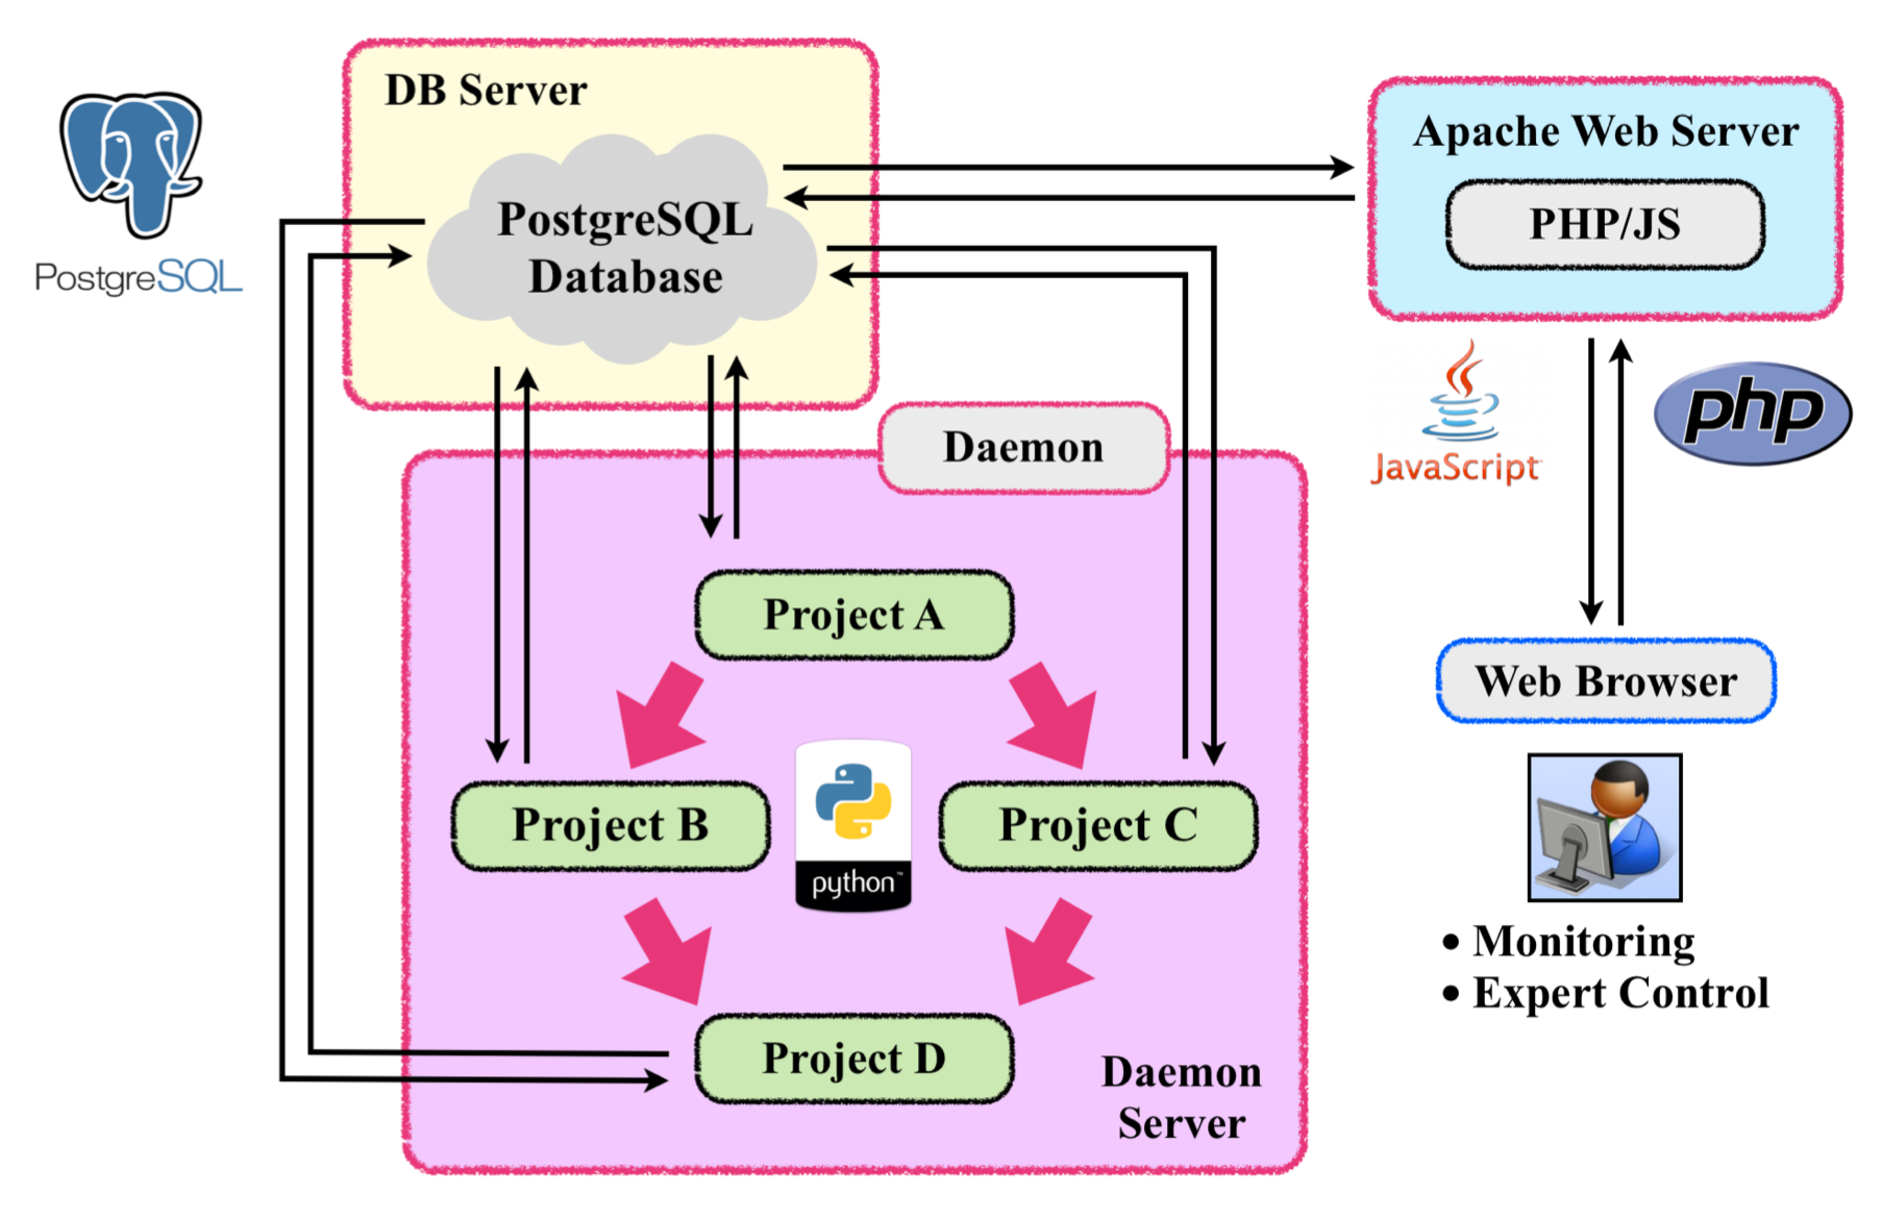
\includegraphics[width=14.5cm]{./img/PUB_Model.pdf}
\caption{ An abstract drawing that shows how data flows into and from the
{\psql} database within {\pubs} framework. Each project and daemon process
all talk to the database server. The {\php} web-interface provides monitoring
and project management tools.}
\label{pubs:model:model}
\end{center}\end{figure}


\subsection{Web Monitoring And Process Management}
\label{pubs:model:monitor}

Figure\ref{pubs:model:model} shows a brief data flow from and into the 
{\psql} database. As described in Sec.\ref{pubs:model:project} and
\ref{pubs:model:daemon}, each project and daemon accesses the database
server individually. In addition to the project execution framework, 
{\pubs} provides {\php} based monitoring and management interface through 
a web server machine and end-user's web browser application. Accordingly
there is a database connection between the web server and {\psql} server
machines.

The capability to monitor each projects' status through a web browser is
quite useful for a routine inspection, such as shifters' check list.
Similarly a formatted control pannel for managing project
execution is useful for experts to take action without logging into the
machine. The details of {\php} implementation is quite experiment specific, 
and the MicroBooNE usage will be discussed in Ch.\ref{dstream}. 


\section{{\psql} Functions}
\label{pubs:psql}

Now that we spent many pages to discuss about the {\pubs} model, let's talk
about something real and practical. This section presents a list of {\pubs} 
functions implemented on the {\psql} server. About a half of them are for
experts' use (in fact mostly for daemon and automated scripts since human
hands are one of last things to be trusted), and the other half is for
project scripts to use. 

If you are a project code developper and do not find a function of your
need, please contact the author and he will be more than happy to assist
how the existing function may solve the problem or implement a brand
new function to make your life easier.

\subsection{Project Information/Status Query}
These are functions that can be used by projects upon execution. That being
said, however, it is {\bf \color{blue} strongly recommended to use {\python} 
API within {\pubs} to execute these functions}. They should not be executed
from {\psql} interpreter or directly executing from an SQL script. If the 
list lacks any function needed for a project execution, please contact the 
author with a request. Functions and corresponding {\python} API will be 
provided.
\begin{itemize}
  \item {\bf DoesTableExist( name TEXT )}
    \begin{itemize}
      \item Checks if a table of the {\it name} exists or not in the database
        by checking the administrative master table. The table name is required
        to be in lowercase (there is no uppercase vs. lowercase in distinction
        among {\psql} server objects).
    \end{itemize}
  \item {\bf DoesProjectExist( name TEXT )}
    \begin{itemize}
      \item Checks if a project with the {\it name} exists or not in the 
        database. In addition to DoesTableExist(), this function checks
        if a specified project exists or not.
    \end{itemize}
  \item {\bf GetRunTimeStamp( Run INT, SubRun INT )}
    \begin{itemize}
      \item A function to retrieve the run start and end time stamp.
    \end{itemize}
  \item {\bf ProjectResource( name TEXT )}
    \begin{itemize}
      \item Returns a project resource (information needed for an execution)
        for a specified project name.
    \end{itemize}
  \item {\bf IncreaseProjSequence( name TEXT, run INT, subrun INT, nseq
    SMALLINT, status SMALLINT) }
    \begin{itemize}
      \item Increase number of sequence count in the specified project table
        for the specified run/sub-run number combination. Input status code 
        is used for all newly created TaskIDs.
    \end{itemize}
  \item {\bf UpdateProjStatus( name TEXT, run INT, subrun INT, seq SMALLINT,
    status SMALLINT, data TEXT)}
    \begin{itemize}
      \item Update the specified project's status for the specified TaskID. 
        At the same time, a TaskID specific data can be also stored although
        that is not necessary (by default the last argument is set to NULL).
    \end{itemize}
  \item {\bf GetProjectData( name TEXT, run INT, subrun INT, seq SMALLINT )}
    \begin{itemize}
      \item Retrieve project data for a specified TaskID. Only accessible to
        The data from the latest version number to avoid a confusion (and
        hence version number cannot be specified).
    \end{itemize}
  \item {\bf GetRuns( name TEXT, status SMALLINT) }
    \begin{itemize}
      \item Returns a table of TaskID (run, sub-run, seq., project-version) 
        for which the specified project carries the specified status code.
    \end{itemize}
  \item {\bf GetRuns( TEXT[]::ARRAY, SMALLINT[]::ARRAY )}
    \begin{itemize}
      \item Similar to GetRuns and it returns a table of run/sub-run number 
      combinations for which all specified projects in the first argument
      carry specified status code in the second argument. This function
      is useful to obtain a list of run/sub-run numbers across multiple
      project tables for specific combination of status code. Because 
      a sequence number is project dependent, it returns run/sub-run for
      which all belonging sequence status uniquely matches with the specified
      status code.
    \end{itemize}

\end{itemize}


\subsection{Functions For Project Management}
These are functions to be used by daemon process to maintaine/running the
projects. In principle these should not be used by a project execution. 
\begin{itemize}
  \item {\bf RemoveProject( name TEXT )} 
    \begin{itemize}
      \item Properly remove a project: drop a project table and remove the
        project information entry from the ProcessTable.
    \end{itemize}
  \item {\bf ListProject()}
    \begin{itemize}
      \item List all projects with the latest version number from ProcessTable.
    \end{itemize}
  \item {\bf ListEnabledProject()}
    \begin{itemize}
      \item List currently enabled project information with the latest version
        number from the ProcessTable.
    \end{itemize}
  \item {\bf DefineProject( name TEXT, command TEXT, frequency INT, email TEXT,
    start\_run INT, start\_subrun INT, resource HSTORE, enabled BOOLEAN )}
    \begin{itemize}
      \item A function to define a new project. It takes in project information
        and registers into the ProcessTable. It also calls {\bf MakeProjTable}
        function to create a project table.
    \end{itemize}
  \item {\bf MakeProjTable( name TEXT )}
    \begin{itemize}
      \item Function dedicated to create a project table. This function is
        to be called by {\bf DefineProject} and not to be called by hand!
    \end{itemize}
  \item {\bf UpdateProjectConfig( name TEXT, command TEXT, frequency INT, email
    TEXT, resource HSTORE, enabled BOOLEAN, version INT)}
    \begin{itemize}
      \item A function to alter and update project configuration. As seen in
        the function arguments, start run/sub-run number cannot be altered by
        design.
    \end{itemize}
  \item {\bf ProjectVersionUpdate( name TEXT, command TEXT, frequency INT,
    email TEXT, run INT, subrun INT, resource HSTORE, enable BOOLEAN)}
    \begin{itemize}
      \item Increment the project version number and store new project
        information. Unlike {\bf UpdateProjectConfig}, this function can
        register any project information as there will be a distinct row
        to be inserted in the ProcessTable.
    \end{itemize}
  \item {\bf GetVersionRunRange( name TEXT )}
    \begin{itemize}
      \item For a specified project name, returns multiple result sets each
        representing a specific run number range with the corresponding
        project version number.
    \end{itemize}
  \item {\bf InsertIntoProjTable( name TEXT, run INT, subrun INT )}
    \begin{itemize}
      \item Insert a new run/sub-run number entry into a project table with
        the default status code of 1. The latest version number for the
        subject run/sub-run is also taken from the ProcessTable.
    \end{itemize}
  \item {\bf OneProjectRunSynch()}
    \begin{itemize}
      \item Make sure one particular project table has run/sub-run 
        numbers that currently appears in the MainRun table and above
        the specified run/subrun numbers in the argument.
    \end{itemize}
  \item {\bf AllProjectRunSynch()}
    \begin{itemize}
      \item Make sure all project table has run/sub-run numbers that 
        currently appears in the MainRun and above the specified start
        run/sub-run numbers in the project information.
    \end{itemize}
  \item {\bf ProjectInfo(name TEXT, ver INT)}
    \begin{itemize}
      \item Returns project information for a specified version number.
        By default the version number does not need to be specified.
        If not given, it is set to the latest version number. This function
        is used to run a project via daemon.
    \end{itemize}
\end{itemize}

\subsection{Admin Functions}
Functions prepared for the top-level administrative purposes. These functions
should be executed by database admins only.
\begin{itemize}
  \item {\bf RemoveProcessDB()}
    \begin{itemize}
      \item ``Properly'' remove {\it everything}. This function drops all
        projects registered in ProcessTable using {\bf RemoveProject} 
        function. Then it drops an empty ProcessTable.
    \end{itemize}
  \item {\bf CreateProcessTable()}
    \begin{itemize}
      \item A simple function to create the ProcessTable.
    \end{itemize}
  \item {\bf CreateTestRunTable()}
    \begin{itemize}
      \item A function to create ``fake'' MainRun table. This is for 
        development work, and not for an official operation. In the official
        production, MainRun table is slave-copied from the configuration
        database automatically.
    \end{itemize}
  \item {\bf InsertIntoTestRunTable( Run INT, SubRun INT, TimeStart TIMESTAMP, TimeEnd TIMESTAMP )}
    \begin{itemize}
      \item A function to insert a new entry into the ``fake'' MainRun table.
        This is not meant to be used for the offial production.
    \end{itemize}
  \item {\bf FillTestRunTable( NRuns INT, NSubRuns INT)}
    \begin{itemize}
      \item A function to fill the ``fake'' MainRun table with multiple entries
        at once. It fills the table with NRuns, each with NSubRuns.
    \end{itemize}
  \item {\bf CheckDBIntegrity()}
    \begin{itemize}
      \item Returns a boolean after checking the process DB integrity. 
        In particular it checks if ProcessTable exists or not, and then
        checks if all projects registered in ProcessTable have own project
        tables.
    \end{itemize}
\end{itemize}





\section{{\python} Software Framework}
\label{pubs:python}
The ``software framework'' part of {\pubs}, which provides the code base 
for application development, is really in {\python}. This section describes
 {\python} tools in {\pubs} that can be used to develop a project execution 
code and set up the data processing chain of multiple projects.

There are three (somewhat) big {\python} modules in {\pubs}:
\begin{itemize}
  \item {\pubutil} $\ldots$ basic framework tools
  \item {\pubdbi} $\ldots$ generic database interface based using {\psycopg}
  \item {\dstream} $\ldots$ data processing framework toolkit
\end{itemize}
A project code developer interfaces with {\dstream} directly while that itself 
depends on basic tools defined in {\pubutil} and {\pubdbi}. We go over each 
of these in the following sections. 

\subsection{{\pubutil}: Basic Toolkit}
This module introduce 3 objects: {\publogger}, {\pubsmtp}, and {\pubexception}.
They are framework logging tool, email sender function via SMTP, and a base exception
class definition. 

\subsubsection{{\publogger} $\ldots$ Logging Module}
This is the framework logger tool, and uses a popular {\python}'s logging module.
{\publogger} is a factory class that can instansiate an individual logger instance
with a specific message format and a choice of stream: either {\stdout}/{\stderr} or
output file stream. 

Each logger instance created by {\publogger} factory has a unique name, and 
can be instantiated by a factory function call:
\begin{lstlisting}
  >>> pubs_logger.get_logger('my_logger')
\end{lstlisting}
for a logger named ``my\_logger''. {\publogger} keeps track of all created loggers 
in its class variable {\ttfamily \_loggers}. When there is a request for a logger
with the same name created in the past, it returns the same instance.
\begin{lstlisting}
  >>> from pub_util import pub_logger
  >>> pub_logger.get_logger('a')
  [ INFO    ] pub_logger (L: 81 ) >> {_add_logger} OPENED LOGGER a
  <logging.Logger object at 0x10b903f90>
  >>> pub_logger.get_logger('a')
  <logging.Logger object at 0x10b903f90>
  >>>
\end{lstlisting}

As you might expect in any similar tool, {\publogger} has several message levels:
debug, info, warning, error, and critical. The default message level is set via
shell environment variable {\ttfamily \$PUB\_LOGGER\_LEVEL}, which is automatically
set in {\ttfamily setup.sh} configuration script. You may change the level if you
wish. You do not have to change the configuration script, but instead just change
the shell environment variable in any way you want (for instance by hand on your
terminal instead of sourcing a script). The set shell environment value is parsed 
in {\ttfamily pub\_util/pub\_env.py} script to an appropriate value. 
Similarly, the stream destination (either {\stdout} or file stream) is
set via shell environment variable {\ttfamily \$PUB\_LOGGER\_DRAIN}, again set
automatically in {\ttfamily setup.sh}. In case the drain is chosen to be a text
file stream, {\ttfamily \$PUB\_LOGGER\_FILE\_LOCATION} environment variable's value
is used as the log file location.

Each message level has a dedicated logger function call to parse an output message
through your logger. Here is an example of formatted output :
\begin{lstlisting}
  >>> a.debug('This is debug')
  [ DEBUG   ] <stdin> (L: 1  ) >> {<module>} This is debug
  >>> a.info('This is info')
  [ INFO    ] <stdin> (L: 1  ) >> {<module>} This is info
  >>> a.warning('This is warning')
  [ WARNING ] <stdin> (L: 1  ) >> {<module>} This is warning
  >>> a.error('This is error')
  [ ERROR   ] <stdin> (L: 1  ) >> {<module>} This is error
  >>> a.critical('This is critical')
  [ CRITICAL] <stdin> (L: 1  ) >> {<module>} This is critical
\end{lstlisting}
The logger specifies the message level, and prints out three more information in
addition to the sent message by the caller. The first `$<$stdin$>$' tells where the
message is sent from. `(L: 1  )' tells us which line in the caller's module code
this function is called from. Then `\{$<$module$>$\}' tells us the name of the
caller's module. In the above example, this is called from the main, and hence
it is not really useful. However, these information help us to track down problems
easily as you can identify where each function call is made. For instance, running
{\ttfamily ds\_daemon.py} to test the installation (see Sec.\ref{prep:pubs:daemon}),
you have probably seen this message:
\begin{lstlisting}
  [ DEBUG   ] ds_daemon (L: 128) >> {load_projects} Updating project dummy_daq ...
\end{lstlisting}
 This menas that a logger function ``debug'' was called by a function 
{\ttfamily load\_projects} and the exact location is in line number 128 of the 
module code {\ttfamily ds\_daemon.py}. 

\subsubsection{{\pubsmtp} $\ldots$ Simple SMTP Protocole}
{\pubsmtp} is a simple function that uses the Simple Mail Transfer Protocole to
send an email message. One can specify the recipients, subject and text message
to be sent. By default, the SMTP account, server address (and port), and password
 are taken from, again, shell environment variables: {\ttfamily \$PUB\_SMTP\_ACCT}, 
{\ttfamily \$PUB\_SMTP\_SRVR}, and {\ttfamily \$PUB\_SMTP\_PASS} respectively.
These are currently set to an email account created for a common use. You may change
this to your account if you wish, or we use an official account when in production.

\subsubsection{{\pubexception} $\ldots$ Simple Exception}
This is an exception class that inherits from the base {\python} {\ttfamily Exception}.
It is nothing special but takes an error message in the constructor argument.
Only purpose is to have a common exception within {\pubs} so that we can catch {\pubs}
specific exception.

\subsection{{\pubdbi}: Generic DB Interface}
{\pubdbi} module defines client tools used to interface with {\psql} database server.
In particular it contains following classes
\begin{itemize}
  \item {\pubdbconn} $\ldots$ for connecting database server
  \item {\pubdbdata} $\ldots$ class that encapsulates connection information 
  \item {\pubdbexception} $\ldots$ exception dedicated for {\pubdbi} module
  \item {\pubdbreader} $\dots$ ``read-only'' database query API instantiated by {\pubdbconn}
  \item {\pubdbwriter} $\dots$ ``read/write'' database query API instantiated by {\pubdbconn}
\end{itemize}
Note that a project code developer should use a wrapper API that is under {\dstream}.
This section covers base components that are usually hidden in behind.
OK let's go through them. Hope I can contribute to your good sleep.

\subsubsection{{\pubdbconn} database connection factory}
This is a factory class that connects to the database using {\psycopg} and generate
a connection cursor ({\ttfamily psycopg2.cursor}) for {\pubdbreader} and {\pubdbwriter}
APIs.

\subsection{{\dstream}: Data Processing Framework}


\section{{\php}-based Web Interface}
\label{pubs:php}
\input{./src/PUBS/php}




% PUBS
\chapter{MicroBooNE Implementation}
\label{dstream}

This chapter describes about building blocks of {\pubs} framework. Sec.\ref{pubs:model} covers the data process management model and the framework design.
Three following sections \ref{pubs:psql}, \ref{pubs:python}, \ref{pubs:php}
 cover {\psql}, {\python}, and {\php} components as building blocks of the 
framework respectively. More practical development how-to's are discussed 
in the next chapter.

\section{Data Processing Model}
\label{pubs:model}

{\pubs} is a data processing software framework that supports a specific
data process model implementation by application developers. In particular,
it has following features:
\begin{itemize}
  \item Use {\psql} for process management
  \item Supports {\python} code development for implementation
  \item Provides {\php} toolkit for application management and monitoring
\end{itemize}
This section describes a generic idea of {\pubs} data processing model.

\subsection{Project: A Unit Task of Data Processing}
\label{pubs:model:project}
A typical model of data processing is a well defined chain of processes
in which a particular process is triggered by a completion or an initiation
of another process. For instance, the end of running DAQ may trigger a file
transfer protocole to move a raw data file to a storage server. In {\pubs},
each of such processes is called a {\it project}. 

\subsubsection{Project Status}
Each {\pubs} project carries a specific {\it status} code represented
by an integer. A unit of status is defined by, in case of MicroBooNE, a
unique combination of four integeres: run, sub-run, {\it sequence} 
(or simply {\it seq}), and the project version number. This combination is
referred to as {\it TaskID} in this document. A run and sub-run numbers 
defines a boundary of data taking  defined by a DAQ as you might guess. 
A sequence number, on the other hand, is a possible sub-set of run and 
sub-run number combination, and is defined by a project. It is there to 
support some projects that may need to sub-divide a process to deal with 
a particular DAQ run. As its name says, the project version is an integer
representing different version of the same project. 

Each {\pubs} project carries a status for each TaskID. Special status code 
1 is reserved to represent the initial status for any project. Similarly, 
code 0 is reserved to represent the completion status for any 
project. Any other integer values may be used to represent various status 
which meaning may be defined by a project.

\subsubsection{Project Version}
One important feature of data processing framework is an ability to roll-back
and re-process some older data files. Reprocessing of data is supported in
{\pubs}, but it requires to change a project version number. The basic 
assumption for forcing the version update for re-processing is that something
must have changed to roll back and re-process data. 
\begin{figure}[ht]\begin{center}
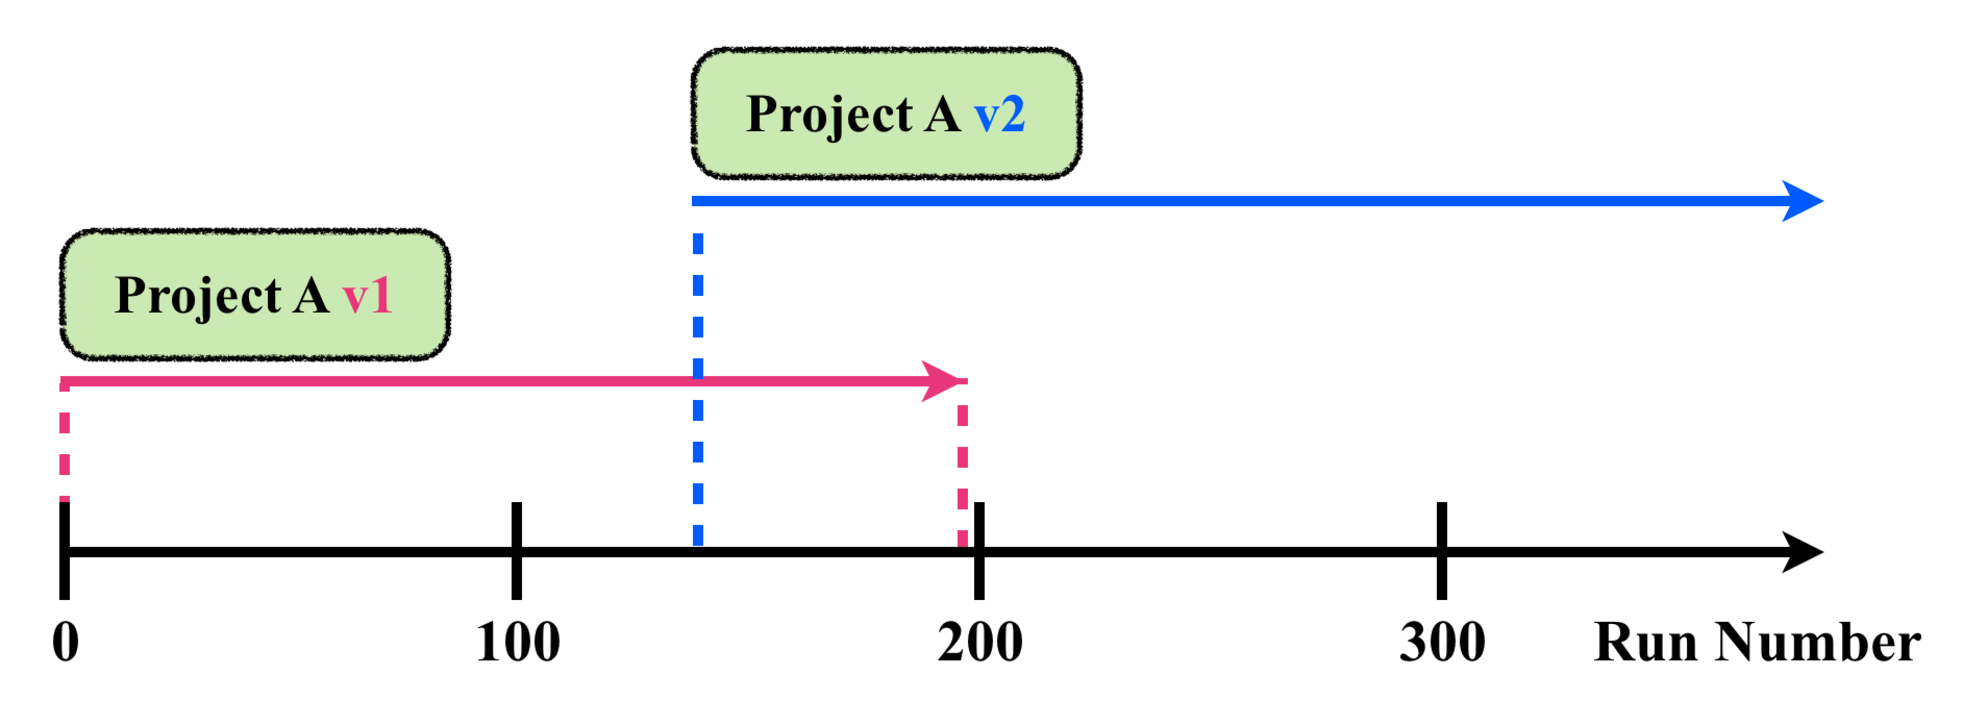
\includegraphics[width=14cm]{./img/PUB_ProjectVersion.pdf}
\caption{ Example diagram showing how project version may be used. 
The horizontal axis shows the time in the unit of a run number 
(sub-run number ignored for simplicity). The diagram shows that the 1st 
version of project A processing data up to around run 200. Then the updated 
2nd version starts re-processing runs just before around run 150 and takes 
over to process all future runs.}
\label{pubs:model:version}
\end{center}\end{figure}
Figure\ref{pubs:model:version} shows an example of reprocessing associated
with a specific project's version update.


\subsubsection{Project Table}
Each project status is stored in {\psql} database table with a name same
as the project's name, called a project table. For this reason, {\bf a 
project name must be unique}. A project table contains several information 
per unique combination of run, sub-run, seq numbers, and they are shown below 
with corresponding {\psql} data type.
\begin{itemize}
\item Run $\ldots$ INT $\ldots$ DAQ run number
\item SubRun $\ldots$ INT $\ldots$ DAQ sub-run number
\item Seq $\ldots$ SMALLINT $\ldots$ project sequence number
\item Status $\ldots$ SMALLINT $\ldots$ project status code
\item Data $\ldots$ TEXT $\ldots$ Generic ``data'' associated with a particular run, sub-run combination
\item ProjectVer $\ldots$ SMALLINT $\ldots$ a version number for a project
\end{itemize}
A project may record some ``data'' in string representation for each TaskID.
However, it is recommended to avoid to store such information when possible 
as this makes the table size to become larger. Finally, as mentioned before,
a project is allowed to have a different version number. 

\subsubsection{Project Execution Model}
Each project is expected to have a single {\python} script to be executed.
This {\python} script should fetch an array of target TaskID from the 
database based on a status code. Depending on the status code, then, the
script may take a certain action, and possibly update the status code in the
database upon success. In short, the status code is used as a trigger for
a specific action by projects. 

Now, information needed to execute each such script is called {\it project
information}, and is stored in a separate database table called the 
{\it ProcessTable}. In the next section, we discuss about this table and
also a machinary to automatically execute a project's {\python} script
using a daemon tool.

\subsection{ProcessTable And Daemon Execution}
\label{pubs:model:daemon}
Information about individual project is stored in a dedicated database
table called ``ProcessTable''. Unlike project tables that exist one per
project, this is a unique table in the database that holds all projects'
information. The table schema is shown below:
\begin{itemize}
  \item ID $\ldots$ SERIAL $\ldots$ a unique integer key for each project
  \item Project $\ldots$ TEXT $\ldots$ the name of a project
  \item ProjectVer $\ldots$ SMALLINT $\dots$ the version number of a project
  \item Command $\ldots$ TEXT $\ldots$ a project execution command to be run
  \item Frequency $\ldots$ INT $\ldots$ latency in seconds between each execution of a project
  \item EMail $\ldots$ TEXT $\ldots$ email contact(s) in case of a trouble
  \item StartRun $\ldots$ INT $\ldots$ the first run-number to be processed
  \item StartSubRun $\ldots$ INT $\ldots$ the first sub-run number to be processed
  \item Resource $\ldots$ HSTORE $\ldots$ a dynamic string-to-string map data container
  \item Enabled $\ldots$ BOOLEAN $\ldots$ a boolean flag for project execution (only if it is true)
  \item Running $\ldots$ BOOLEAN $\ldots$ a boolean flag enabled during project execution
  \item LogTime $\ldots$ TIMESTAMP $\ldots$ a time-stamp logged per entry update
\end{itemize}
where, among many self-descriptive columns, ``Resource'' column holds HSTORE
type variable that can be used to store any project-specific information.
Such information includes, for example, the path to a specific data directory
and expected file name format that requires run and sub-run numbers such as
\begin{center}
 {\ttfamily Run\%05d\_SubRun\%03d.bin}.
\end{center}
with which your project can figure out the expected file name for a given
TaskID (i.e. run and sub-run numbers). 

Note that storing such information in ProcessTable is much lighter than 
storing the actual filename in a project table's ``Data'' column because 
the ``Data'' column stores information for every single TaskID while 
ProcessTable entry is made only one per project. Again, store as much
information as possible in ProcessTable and avoid using ``Data'' column
of a project table when possible.

\subsubsection{Daemon: Master Scheduler}
An execution of a project should be as simple as:
\begin{lstlisting}
  > python my_project.py
\end{lstlisting}
where my\_project.py is the executor of a project. In {\pubs}, however,
there is a simple daemon project management tool that periodically 
looks up the ProcessTable and executes the enabled projects in parallel. 
So it is a lot like {\ttfamily cron} in Unix/Linux but with a process
manager aspect.  

The daemon process is responsible for project management: it keeps track
of history of running each project, and it ensures its resoure usage. 
The project information is updated every 120 seconds (configurable) and 
synchronized with the ProcessTable contents in the database. An expert
can impose a change in project information without interrupting the daemon
process. Another important role of the daemon is to keep the integrity of
the DAQ's run table with all enabled projects' table. Once in every 300
seconds (configurable), the daemon process synchronizes run and sub-run
number entries in each project table and match with the DAQ run table.

That being said, it is extremely important that each project is a truly
modulated action, and does not depend on an execution by the daemon. In
other words, one should be able to always run a project by simply invoking
from a command line. This allows us to take any emergency treatment when,
somehow, the daemon procedure cannot be used.

\begin{figure}\begin{center}
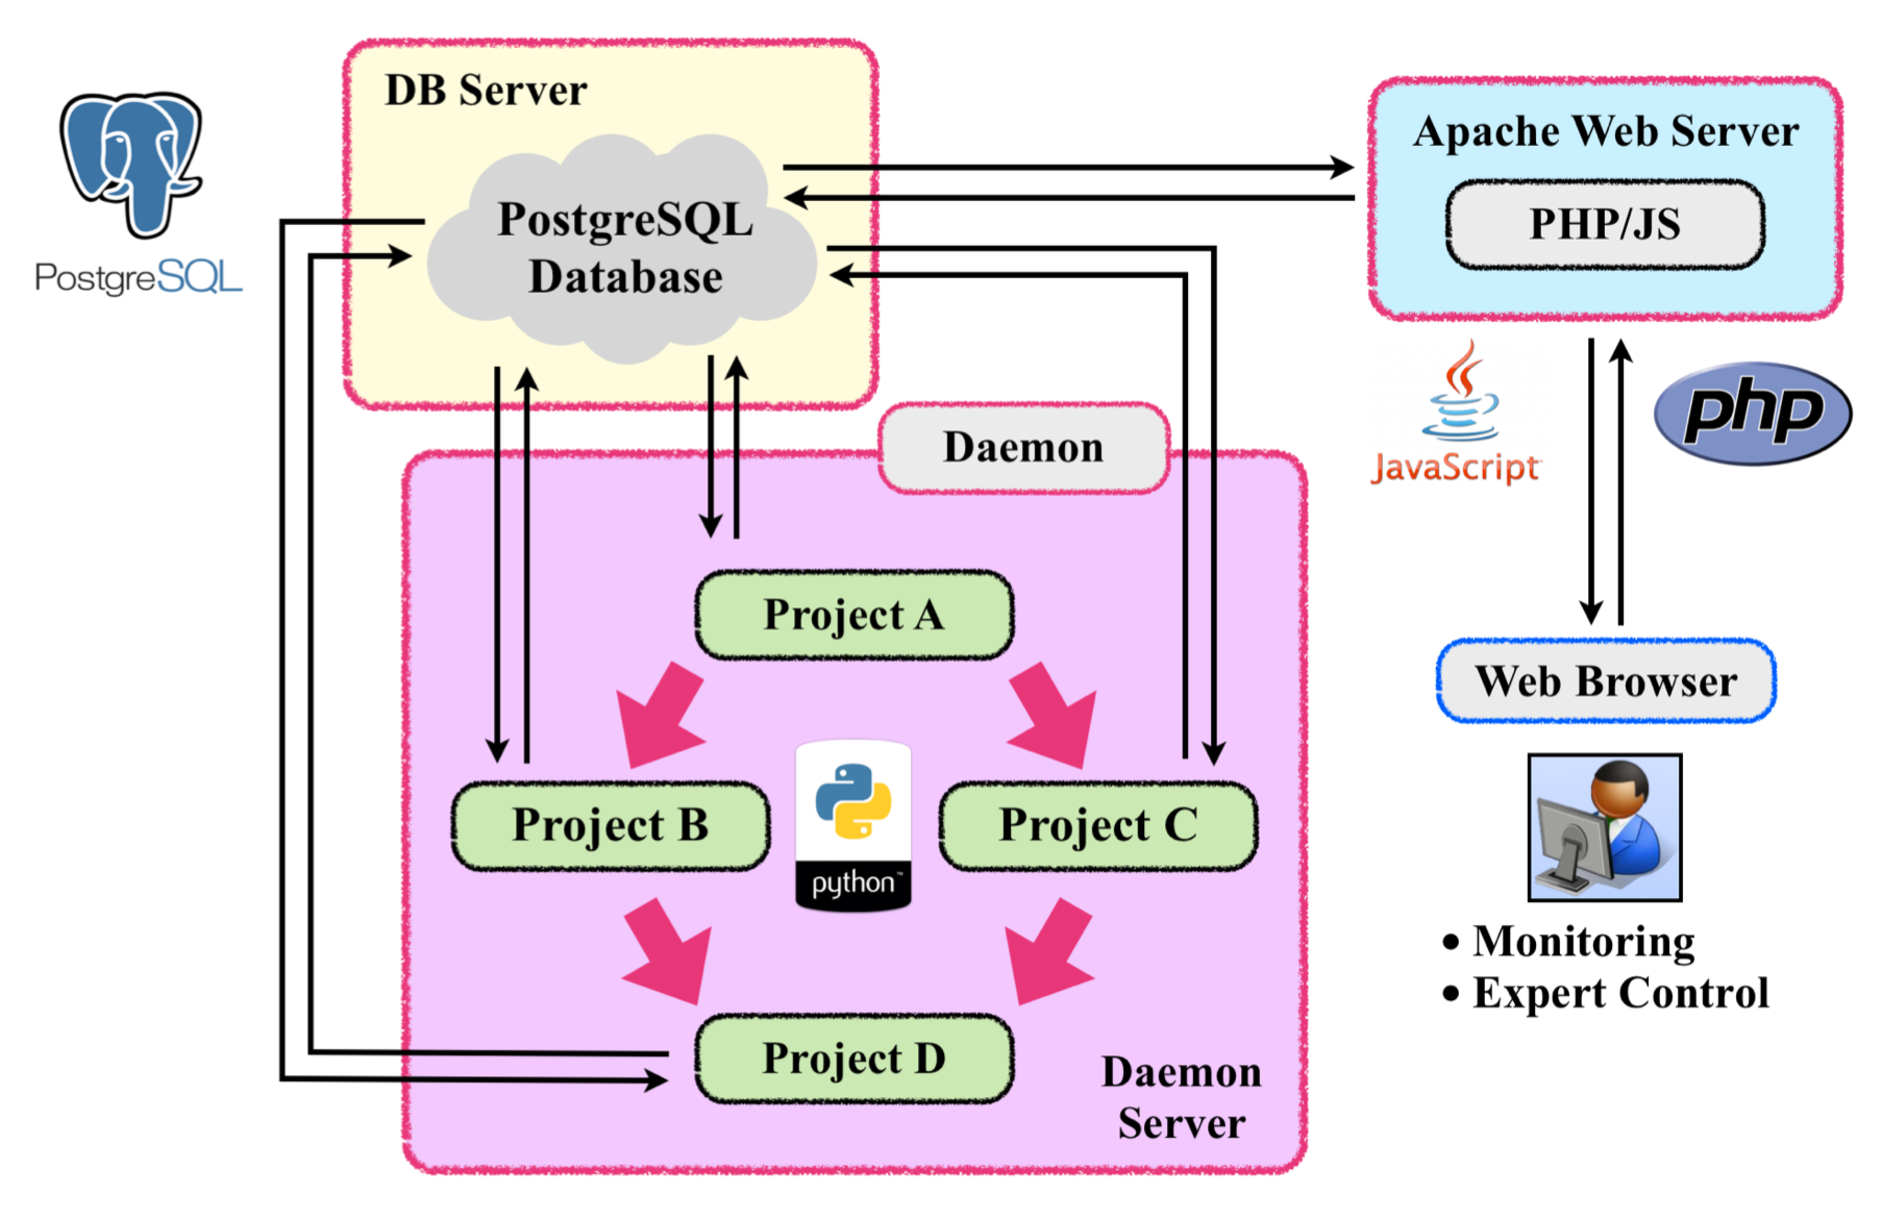
\includegraphics[width=14.5cm]{./img/PUB_Model.pdf}
\caption{ An abstract drawing that shows how data flows into and from the
{\psql} database within {\pubs} framework. Each project and daemon process
all talk to the database server. The {\php} web-interface provides monitoring
and project management tools.}
\label{pubs:model:model}
\end{center}\end{figure}


\subsection{Web Monitoring And Process Management}
\label{pubs:model:monitor}

Figure\ref{pubs:model:model} shows a brief data flow from and into the 
{\psql} database. As described in Sec.\ref{pubs:model:project} and
\ref{pubs:model:daemon}, each project and daemon accesses the database
server individually. In addition to the project execution framework, 
{\pubs} provides {\php} based monitoring and management interface through 
a web server machine and end-user's web browser application. Accordingly
there is a database connection between the web server and {\psql} server
machines.

The capability to monitor each projects' status through a web browser is
quite useful for a routine inspection, such as shifters' check list.
Similarly a formatted control pannel for managing project
execution is useful for experts to take action without logging into the
machine. The details of {\php} implementation is quite experiment specific, 
and the MicroBooNE usage will be discussed in Ch.\ref{dstream}. 


\section{{\psql} Functions}
\label{pubs:psql}

Now that we spent many pages to discuss about the {\pubs} model, let's talk
about something real and practical. This section presents a list of {\pubs} 
functions implemented on the {\psql} server. About a half of them are for
experts' use (in fact mostly for daemon and automated scripts since human
hands are one of last things to be trusted), and the other half is for
project scripts to use. 

If you are a project code developper and do not find a function of your
need, please contact the author and he will be more than happy to assist
how the existing function may solve the problem or implement a brand
new function to make your life easier.

\subsection{Project Information/Status Query}
These are functions that can be used by projects upon execution. That being
said, however, it is {\bf \color{blue} strongly recommended to use {\python} 
API within {\pubs} to execute these functions}. They should not be executed
from {\psql} interpreter or directly executing from an SQL script. If the 
list lacks any function needed for a project execution, please contact the 
author with a request. Functions and corresponding {\python} API will be 
provided.
\begin{itemize}
  \item {\bf DoesTableExist( name TEXT )}
    \begin{itemize}
      \item Checks if a table of the {\it name} exists or not in the database
        by checking the administrative master table. The table name is required
        to be in lowercase (there is no uppercase vs. lowercase in distinction
        among {\psql} server objects).
    \end{itemize}
  \item {\bf DoesProjectExist( name TEXT )}
    \begin{itemize}
      \item Checks if a project with the {\it name} exists or not in the 
        database. In addition to DoesTableExist(), this function checks
        if a specified project exists or not.
    \end{itemize}
  \item {\bf GetRunTimeStamp( Run INT, SubRun INT )}
    \begin{itemize}
      \item A function to retrieve the run start and end time stamp.
    \end{itemize}
  \item {\bf ProjectResource( name TEXT )}
    \begin{itemize}
      \item Returns a project resource (information needed for an execution)
        for a specified project name.
    \end{itemize}
  \item {\bf IncreaseProjSequence( name TEXT, run INT, subrun INT, nseq
    SMALLINT, status SMALLINT) }
    \begin{itemize}
      \item Increase number of sequence count in the specified project table
        for the specified run/sub-run number combination. Input status code 
        is used for all newly created TaskIDs.
    \end{itemize}
  \item {\bf UpdateProjStatus( name TEXT, run INT, subrun INT, seq SMALLINT,
    status SMALLINT, data TEXT)}
    \begin{itemize}
      \item Update the specified project's status for the specified TaskID. 
        At the same time, a TaskID specific data can be also stored although
        that is not necessary (by default the last argument is set to NULL).
    \end{itemize}
  \item {\bf GetProjectData( name TEXT, run INT, subrun INT, seq SMALLINT )}
    \begin{itemize}
      \item Retrieve project data for a specified TaskID. Only accessible to
        The data from the latest version number to avoid a confusion (and
        hence version number cannot be specified).
    \end{itemize}
  \item {\bf GetRuns( name TEXT, status SMALLINT) }
    \begin{itemize}
      \item Returns a table of TaskID (run, sub-run, seq., project-version) 
        for which the specified project carries the specified status code.
    \end{itemize}
  \item {\bf GetRuns( TEXT[]::ARRAY, SMALLINT[]::ARRAY )}
    \begin{itemize}
      \item Similar to GetRuns and it returns a table of run/sub-run number 
      combinations for which all specified projects in the first argument
      carry specified status code in the second argument. This function
      is useful to obtain a list of run/sub-run numbers across multiple
      project tables for specific combination of status code. Because 
      a sequence number is project dependent, it returns run/sub-run for
      which all belonging sequence status uniquely matches with the specified
      status code.
    \end{itemize}

\end{itemize}


\subsection{Functions For Project Management}
These are functions to be used by daemon process to maintaine/running the
projects. In principle these should not be used by a project execution. 
\begin{itemize}
  \item {\bf RemoveProject( name TEXT )} 
    \begin{itemize}
      \item Properly remove a project: drop a project table and remove the
        project information entry from the ProcessTable.
    \end{itemize}
  \item {\bf ListProject()}
    \begin{itemize}
      \item List all projects with the latest version number from ProcessTable.
    \end{itemize}
  \item {\bf ListEnabledProject()}
    \begin{itemize}
      \item List currently enabled project information with the latest version
        number from the ProcessTable.
    \end{itemize}
  \item {\bf DefineProject( name TEXT, command TEXT, frequency INT, email TEXT,
    start\_run INT, start\_subrun INT, resource HSTORE, enabled BOOLEAN )}
    \begin{itemize}
      \item A function to define a new project. It takes in project information
        and registers into the ProcessTable. It also calls {\bf MakeProjTable}
        function to create a project table.
    \end{itemize}
  \item {\bf MakeProjTable( name TEXT )}
    \begin{itemize}
      \item Function dedicated to create a project table. This function is
        to be called by {\bf DefineProject} and not to be called by hand!
    \end{itemize}
  \item {\bf UpdateProjectConfig( name TEXT, command TEXT, frequency INT, email
    TEXT, resource HSTORE, enabled BOOLEAN, version INT)}
    \begin{itemize}
      \item A function to alter and update project configuration. As seen in
        the function arguments, start run/sub-run number cannot be altered by
        design.
    \end{itemize}
  \item {\bf ProjectVersionUpdate( name TEXT, command TEXT, frequency INT,
    email TEXT, run INT, subrun INT, resource HSTORE, enable BOOLEAN)}
    \begin{itemize}
      \item Increment the project version number and store new project
        information. Unlike {\bf UpdateProjectConfig}, this function can
        register any project information as there will be a distinct row
        to be inserted in the ProcessTable.
    \end{itemize}
  \item {\bf GetVersionRunRange( name TEXT )}
    \begin{itemize}
      \item For a specified project name, returns multiple result sets each
        representing a specific run number range with the corresponding
        project version number.
    \end{itemize}
  \item {\bf InsertIntoProjTable( name TEXT, run INT, subrun INT )}
    \begin{itemize}
      \item Insert a new run/sub-run number entry into a project table with
        the default status code of 1. The latest version number for the
        subject run/sub-run is also taken from the ProcessTable.
    \end{itemize}
  \item {\bf OneProjectRunSynch()}
    \begin{itemize}
      \item Make sure one particular project table has run/sub-run 
        numbers that currently appears in the MainRun table and above
        the specified run/subrun numbers in the argument.
    \end{itemize}
  \item {\bf AllProjectRunSynch()}
    \begin{itemize}
      \item Make sure all project table has run/sub-run numbers that 
        currently appears in the MainRun and above the specified start
        run/sub-run numbers in the project information.
    \end{itemize}
  \item {\bf ProjectInfo(name TEXT, ver INT)}
    \begin{itemize}
      \item Returns project information for a specified version number.
        By default the version number does not need to be specified.
        If not given, it is set to the latest version number. This function
        is used to run a project via daemon.
    \end{itemize}
\end{itemize}

\subsection{Admin Functions}
Functions prepared for the top-level administrative purposes. These functions
should be executed by database admins only.
\begin{itemize}
  \item {\bf RemoveProcessDB()}
    \begin{itemize}
      \item ``Properly'' remove {\it everything}. This function drops all
        projects registered in ProcessTable using {\bf RemoveProject} 
        function. Then it drops an empty ProcessTable.
    \end{itemize}
  \item {\bf CreateProcessTable()}
    \begin{itemize}
      \item A simple function to create the ProcessTable.
    \end{itemize}
  \item {\bf CreateTestRunTable()}
    \begin{itemize}
      \item A function to create ``fake'' MainRun table. This is for 
        development work, and not for an official operation. In the official
        production, MainRun table is slave-copied from the configuration
        database automatically.
    \end{itemize}
  \item {\bf InsertIntoTestRunTable( Run INT, SubRun INT, TimeStart TIMESTAMP, TimeEnd TIMESTAMP )}
    \begin{itemize}
      \item A function to insert a new entry into the ``fake'' MainRun table.
        This is not meant to be used for the offial production.
    \end{itemize}
  \item {\bf FillTestRunTable( NRuns INT, NSubRuns INT)}
    \begin{itemize}
      \item A function to fill the ``fake'' MainRun table with multiple entries
        at once. It fills the table with NRuns, each with NSubRuns.
    \end{itemize}
  \item {\bf CheckDBIntegrity()}
    \begin{itemize}
      \item Returns a boolean after checking the process DB integrity. 
        In particular it checks if ProcessTable exists or not, and then
        checks if all projects registered in ProcessTable have own project
        tables.
    \end{itemize}
\end{itemize}





\section{{\python} Software Framework}
\label{pubs:python}
The ``software framework'' part of {\pubs}, which provides the code base 
for application development, is really in {\python}. This section describes
 {\python} tools in {\pubs} that can be used to develop a project execution 
code and set up the data processing chain of multiple projects.

There are three (somewhat) big {\python} modules in {\pubs}:
\begin{itemize}
  \item {\pubutil} $\ldots$ basic framework tools
  \item {\pubdbi} $\ldots$ generic database interface based using {\psycopg}
  \item {\dstream} $\ldots$ data processing framework toolkit
\end{itemize}
A project code developer interfaces with {\dstream} directly while that itself 
depends on basic tools defined in {\pubutil} and {\pubdbi}. We go over each 
of these in the following sections. 

\subsection{{\pubutil}: Basic Toolkit}
This module introduce 3 objects: {\publogger}, {\pubsmtp}, and {\pubexception}.
They are framework logging tool, email sender function via SMTP, and a base exception
class definition. 

\subsubsection{{\publogger} $\ldots$ Logging Module}
This is the framework logger tool, and uses a popular {\python}'s logging module.
{\publogger} is a factory class that can instansiate an individual logger instance
with a specific message format and a choice of stream: either {\stdout}/{\stderr} or
output file stream. 

Each logger instance created by {\publogger} factory has a unique name, and 
can be instantiated by a factory function call:
\begin{lstlisting}
  >>> pubs_logger.get_logger('my_logger')
\end{lstlisting}
for a logger named ``my\_logger''. {\publogger} keeps track of all created loggers 
in its class variable {\ttfamily \_loggers}. When there is a request for a logger
with the same name created in the past, it returns the same instance.
\begin{lstlisting}
  >>> from pub_util import pub_logger
  >>> pub_logger.get_logger('a')
  [ INFO    ] pub_logger (L: 81 ) >> {_add_logger} OPENED LOGGER a
  <logging.Logger object at 0x10b903f90>
  >>> pub_logger.get_logger('a')
  <logging.Logger object at 0x10b903f90>
  >>>
\end{lstlisting}

As you might expect in any similar tool, {\publogger} has several message levels:
debug, info, warning, error, and critical. The default message level is set via
shell environment variable {\ttfamily \$PUB\_LOGGER\_LEVEL}, which is automatically
set in {\ttfamily setup.sh} configuration script. You may change the level if you
wish. You do not have to change the configuration script, but instead just change
the shell environment variable in any way you want (for instance by hand on your
terminal instead of sourcing a script). The set shell environment value is parsed 
in {\ttfamily pub\_util/pub\_env.py} script to an appropriate value. 
Similarly, the stream destination (either {\stdout} or file stream) is
set via shell environment variable {\ttfamily \$PUB\_LOGGER\_DRAIN}, again set
automatically in {\ttfamily setup.sh}. In case the drain is chosen to be a text
file stream, {\ttfamily \$PUB\_LOGGER\_FILE\_LOCATION} environment variable's value
is used as the log file location.

Each message level has a dedicated logger function call to parse an output message
through your logger. Here is an example of formatted output :
\begin{lstlisting}
  >>> a.debug('This is debug')
  [ DEBUG   ] <stdin> (L: 1  ) >> {<module>} This is debug
  >>> a.info('This is info')
  [ INFO    ] <stdin> (L: 1  ) >> {<module>} This is info
  >>> a.warning('This is warning')
  [ WARNING ] <stdin> (L: 1  ) >> {<module>} This is warning
  >>> a.error('This is error')
  [ ERROR   ] <stdin> (L: 1  ) >> {<module>} This is error
  >>> a.critical('This is critical')
  [ CRITICAL] <stdin> (L: 1  ) >> {<module>} This is critical
\end{lstlisting}
The logger specifies the message level, and prints out three more information in
addition to the sent message by the caller. The first `$<$stdin$>$' tells where the
message is sent from. `(L: 1  )' tells us which line in the caller's module code
this function is called from. Then `\{$<$module$>$\}' tells us the name of the
caller's module. In the above example, this is called from the main, and hence
it is not really useful. However, these information help us to track down problems
easily as you can identify where each function call is made. For instance, running
{\ttfamily ds\_daemon.py} to test the installation (see Sec.\ref{prep:pubs:daemon}),
you have probably seen this message:
\begin{lstlisting}
  [ DEBUG   ] ds_daemon (L: 128) >> {load_projects} Updating project dummy_daq ...
\end{lstlisting}
 This menas that a logger function ``debug'' was called by a function 
{\ttfamily load\_projects} and the exact location is in line number 128 of the 
module code {\ttfamily ds\_daemon.py}. 

\subsubsection{{\pubsmtp} $\ldots$ Simple SMTP Protocole}
{\pubsmtp} is a simple function that uses the Simple Mail Transfer Protocole to
send an email message. One can specify the recipients, subject and text message
to be sent. By default, the SMTP account, server address (and port), and password
 are taken from, again, shell environment variables: {\ttfamily \$PUB\_SMTP\_ACCT}, 
{\ttfamily \$PUB\_SMTP\_SRVR}, and {\ttfamily \$PUB\_SMTP\_PASS} respectively.
These are currently set to an email account created for a common use. You may change
this to your account if you wish, or we use an official account when in production.

\subsubsection{{\pubexception} $\ldots$ Simple Exception}
This is an exception class that inherits from the base {\python} {\ttfamily Exception}.
It is nothing special but takes an error message in the constructor argument.
Only purpose is to have a common exception within {\pubs} so that we can catch {\pubs}
specific exception.

\subsection{{\pubdbi}: Generic DB Interface}
{\pubdbi} module defines client tools used to interface with {\psql} database server.
In particular it contains following classes
\begin{itemize}
  \item {\pubdbconn} $\ldots$ for connecting database server
  \item {\pubdbdata} $\ldots$ class that encapsulates connection information 
  \item {\pubdbexception} $\ldots$ exception dedicated for {\pubdbi} module
  \item {\pubdbreader} $\dots$ ``read-only'' database query API instantiated by {\pubdbconn}
  \item {\pubdbwriter} $\dots$ ``read/write'' database query API instantiated by {\pubdbconn}
\end{itemize}
Note that a project code developer should use a wrapper API that is under {\dstream}.
This section covers base components that are usually hidden in behind.
OK let's go through them. Hope I can contribute to your good sleep.

\subsubsection{{\pubdbconn} database connection factory}
This is a factory class that connects to the database using {\psycopg} and generate
a connection cursor ({\ttfamily psycopg2.cursor}) for {\pubdbreader} and {\pubdbwriter}
APIs.

\subsection{{\dstream}: Data Processing Framework}


\section{{\php}-based Web Interface}
\label{pubs:php}
\input{./src/PUBS/php}




% Bibliography
\bibliographystyle{unsrt}

\bibliography{PUBS}


\end{document}
